\documentclass[review]{elsarticle}

\usepackage{lineno,hyperref}
%\usepackage{lineno}
\modulolinenumbers[5]

\journal{Journal of Theoretical Computer Science}

%%%%%%%%%%%%%%%%%%%%%%%
%% Elsevier bibliography styles
%%%%%%%%%%%%%%%%%%%%%%%
%% To change the style, put a % in front of the second line of the current style and
%% remove the % from the second line of the style you would like to use.
%%%%%%%%%%%%%%%%%%%%%%%

%% Numbered
%\bibliographystyle{model1-num-names}

%% Numbered without titles
%\bibliographystyle{model1a-num-names}

%% Harvard
%\bibliographystyle{model2-names.bst}\biboptions{authoryear}

%% Vancouver numbered
%\usepackage{numcompress}\bibliographystyle{model3-num-names}

%% Vancouver name/year
%\usepackage{numcompress}\bibliographystyle{model4-names}\biboptions{authoryear}

%% APA style
%\bibliographystyle{model5-names}\biboptions{authoryear}

%% AMA style
%\usepackage{numcompress}\bibliographystyle{model6-num-names}
\usepackage{amsmath}
\usepackage{psfrag}
\usepackage{graphicx}
\usepackage{epsfig}
\usepackage{epstopdf}
\usepackage{amssymb}
\usepackage{bm}
\usepackage[dvipsnames]{xcolor}
\usepackage{mathtools}

%% `Elsevier LaTeX' style
\bibliographystyle{elsarticle-num}
%%%%%%%%%%%%%%%%%%%%%%%

\newcommand{\paral}{\; \vert \;}
\newcommand{\myvec}[1]{\overrightarrow{#1}}
\newcommand{\Defeq}{\stackrel{\mathrm{df}}{=}}
\newcommand{\Bnfeq}{::=}
\newcommand{\Co}[1]{\overline{#1}}

%
\newcommand{\Bsep}{\: \mid \: }
\newcommand{\Rule}[2]{\displaystyle{\frac{#1}{#2}}}
\newcommand{\SF}[1]{\mathsf{#1}}
\newcommand{\Act}{\mathsf{Act}}
\newcommand{\Vis}{\mathsf{Vis}}
\newcommand{\ActK}{\mathsf{ActK}}
\newcommand{\Proc}{\mathsf{Proc}}
\newcommand{\Procc}{\mathsf{ProcC}}
\newcommand{\Pred}{\mathsf{Pred}}
\newcommand{\Std}{\mathsf{Std}}
\newcommand{\rms}{\mathrm{S}}
\newcommand{\rmrec}{\mathrm{rec}}
\newcommand{\rmreck}{\mathrm{reck}}
\newcommand{\rmreckR}{\mathrm{reckR}}
\newcommand{\rma}{\mathrm{A}}
\newcommand{\rmp}{\mathrm{P}}
\newcommand{\rmf}{\mathrm{F}}
\newcommand{\rmr}{\mathrm{R}}
\newcommand{\rmfr}{\mathrm{FR}}
\newcommand{\equivS}{\equiv_{\mathrm{S}}}
\newcommand{\SigSA}{\Sigma_{\mathrm{SA}}}
\newcommand{\ltran}[1]{\stackrel{#1}{\longrightarrow}}
\newcommand{\tran}[1]{\stackrel{#1}{\rightarrow}}
\newcommand{\nottran}[1]{\stackrel{#1}{\not\rightarrow}}
\newcommand{\Rtran}[1]{\stackrel{#1}{\rightsquigarrow}}
\newcommand{\notRtran}[1]{\stackrel{#1}{\not\rightsquigarrow}}
\newcommand{\trans}[1]{\stackrel{#1}{\rightarrow}_{\mathrm{S}}}
\newcommand{\Par}{\mid}
\newcommand{\Mid}{\!\mid\!}
\newcommand{\restrict}[1]{\!\setminus\!#1}

\newcommand{\mA}{\mathcal{A}}
\newcommand{\mSA}{\mathcal{SA}}
\newcommand{\mWA}{\mathcal{WA}}
\newcommand{\mAK}{\mathcal{AK}}
\newcommand{\aAK}{\mathcal{(A)K}}
\newcommand{\umAK}{\underline{\mathcal{A}}\mathcal{K}}
\newcommand{\un}[1]{\underline {#1}}
\newcommand{\PI}{\mathcal{PI}}
\newcommand{\rom}[1]{\mbox{\rm{#1}}}

\newcommand{\Nil}{\mathbf{0}}
\newcommand{\New}[1]{\nu#1\: }
\newcommand{\Str}{\equiv}
\newcommand{\stdpred}{\mathsf{std}}
\newcommand{\std}[1]{\mathsf{std}(#1)}
%
\newcommand{\Bch}[2]{\mathsf{before}_{#1}(#2)}

\newcommand{\keys}[1]{\mathsf{keys}(#1)}
\newcommand{\kkey}[1]{\mathsf{k}(#1)}
\newcommand{\key}[1]{[#1]}
\newcommand{\Keys}{\mathcal{K}}
\newcommand{\freshpred}[1]{\mathsf{fsh}[#1]}
\newcommand{\fresh}[2]{\mathsf{fsh}[#1](#2)}

\newcommand{\ta}[1]{\mathsf{ta}(#1)}
\newcommand{\action}[1]{\mathsf{act}(#1)}

\newcommand{\intr}{\mbox{\ $\hat{}$\ }}
%\newcommand{\intr}{\mbox{\; $\widehat{}$\;}}
\newcommand{\sterm}{\mathsf{trm}}
\newcommand{\Sterm}[1]{\sterm(#1)}
\newcommand{\und}[1]{\underline{#1}}
\newcommand{\sqc}{\mathop{\cdot}}
\newcommand{\card}[1]{|#1|}
\newcommand{\bydef}{\stackrel{\emph{def}}{=}}
%
\newcommand{\Angle}[1]{\langle #1 \rangle}
\newcommand{\Tri}{\triangleright}
%\newcommand{\hole}{\bullet}
\newcommand{\hole}{[\ ]}
\newcommand{\rec}[1]{\mathrm{rec}\, #1}
\newcommand{\Rec}[1]{\rec #1 .}
\newcommand{\Rch}{\mathsf{Rch}}
\newcommand{\prune}{\pi}
\newcommand{\Prune}[1]{\prune(#1)}
\newcommand{\Root}[1]{\mathsf{rt}(#1)}

\newcommand{\Bis}{\sim}
\newcommand{\Biss}{\Bis_{\mathsf{S}}}
\newcommand{\Bisf}{\Bis_{\mathsf{F}}}
\newcommand{\Bisfr}{\Bis_{\mathsf{FR}}}
%\newcommand{\Bisu}{\Bis_{\Un}}
\newcommand{\Sim}{\mathcal{S}}
\newcommand{\Rem}{\backslash}
\newcommand{\sqeqt}{\sim}
% rules:
% static rule
\newcommand{\one}{\mbox{(I)}}
\newcommand{\onef}{\mbox{(1)}}
\newcommand{\oner}{\mbox{(1R)}}
% choice rule
\newcommand{\two}{\mbox{(II)}}
\newcommand{\twof}{\mbox{(2)}}
\newcommand{\twor}{\mbox{(2R)}}
% choice axiom
\newcommand{\thr}{\mbox{(III)}}
\newcommand{\thrf}{\mbox{(3)}}
\newcommand{\thrr}{\mbox{(3R)}}
\newcommand{\thrpf}{\mbox{(3\,$'$\!)}}
\newcommand{\thrpr}{\mbox{(3\,$'$\!R)}}
%
%
\newcommand{\Draft}[1]{}
\newcommand{\Comment}[1]{}
\newcommand{\Rev}[1]{{#1}^{-1}}
\newcommand{\rulename}[1]{\textsf{#1}}

\newcommand{\Blue}[1]{\textcolor{blue}{#1}}
\newcommand{\Red}[1]{\textcolor{red}{#1}}
%
%
\newcommand{\DP}{\mathit{DP}}
\newcommand{\Me}{\mathit{Me}}
\newcommand{\Meprime}{\mathit{Me'}}
\newcommand{\MutS}{\mathit{MutS}}
\newcommand{\MutSprime}{\mathit{MutS'}}
\newcommand{\MutL}{\mathit{MutL}}
\newcommand{\MutH}{\mathit{MutH}}
\newcommand{\UvrD}{\mathit{UvrD}}
%

\newtheorem{theorem}{Theorem}
\newtheorem{definition}{Definition}
\newtheorem{remark}{Remark}
\newtheorem{example}{Example}
\newtheorem{proposition}{Proposition}
%
\newcommand{\xxrightarrow}{\xmapsto}

%

\begin{document}

\begin{frontmatter}

\title{Modelling of DNA Mismatch Repair with a reversible process calculus\tnoteref{mytitlenote}}
%\tnotetext[mytitlenote]{Fully documented templates are available in the elsarticle package on \href{http://www.ctan.org/tex-archive/macros/latex/contrib/elsarticle}{CTAN}.}

%% Group authors per affiliation:
\author{Stefan Kuhn}%\fnref{myfootnote}}
\address{School of Computer Science and Informatics, De Montfort University, Leicester, UK}
\ead{stefan.kuhn@dmu.ac.uk}
%\fntext[myfootnote]{Since 1880.}

\author{Irek Ulidowski}%\fnref{myfootnote}}
\address{School of Computing and Mathematical Sciences, University of Leicester, Leicester, UK}
\ead{iu3@leicester.ac.uk}

%\fntext[myfootnote]{Since 1880.}
%% or include affiliations in footnotes:
%\author[mymainaddress,mysecondaryaddress]{Elsevier Inc}
%\ead[url]{www.elsevier.com}

%\author[mysecondaryaddress]{Global Customer Service\corref{mycorrespondingauthor}}
%\cortext[mycorrespondingauthor]{Corresponding author}
%\ead{support@elsevier.com}
%
%\address[mymainaddress]{1600 John F Kennedy Boulevard, Philadelphia}
%\address[mysecondaryaddress]{360 Park Avenue South, New York}

\begin{abstract}
%We have demonstrated in previous work that the Calculus of Covalent Bonding (CCB) can be used to simulate higher-level biochemical processes. This is significant since CCB was originally devised to model organic chemical reactions on a lower level. We are now extending the use of CCB to model another gene repair pathway, DNA Mismatch Repair (MMR). This is a more complex pathway than the Base Excision Repair (BER) which we modelled originally. It involves four proteins and needs a distinction between the two chains in a DNA strand. We demonstrate that we can model this by extending our modelling of BER and that we can do this using the unchanged CCB calculus and operational semantics. We also show that the simulation software developed previously can be used to execute this pathway.
%
%
We have demonstrated in previous work that the Calculus of Covalent Bonding (CCB) can be used to simulate higher-level biochemical processes. This is significant since CCB was originally devised to model lower level organic chemical reactions. In this paper we extend the use of the calculus  to model an important gene repair pathway, namely DNA Mismatch Repair (MMR). This complex pathway involves four helper proteins and needs a distinction between the two chains in a DNA strand. 
In order to achieve this, we extend the calculus by allowing prefixing with collections of bonding sites.
% and its operational semantics by allowing more complex concerted actions transitions.
% We also show that the simulation software developed previously can be used to execute this pathway.
\end{abstract}

\begin{keyword}Reversible computation, Calculus of Covalent Bonding, DNA Mismatch Repair.
%\texttt{elsarticle.cls}\sep \LaTeX\sep Elsevier \sep template
%\MSC[2010] 00-01\sep  99-00
\end{keyword}

\end{frontmatter}

\linenumbers

\section{Introduction}

We have previously introduced a Calculus of Covalent  Bonding (CCB) \cite{KU16,KU2017} to models the formation and breaking of covalent bonds. % in organic molecules. 
CCB contains the possibility to link forming and breaking of bonds, thus enabling integrated, local control of reversibility. This feature allows us to represent both standard reversibility as well as the out-of-causal order reversibility. In order to demonstrate the basics of our calculus we show how to model the autoprotlysis of water, which transfers a proton between two water molecules. 
%Since the reaction takes place in water it is also known as autoprotolysis of water. 
This reversible reaction is shown in Figure~\ref{fig:autoprotolysis}.
%
\begin{figure}
\centering
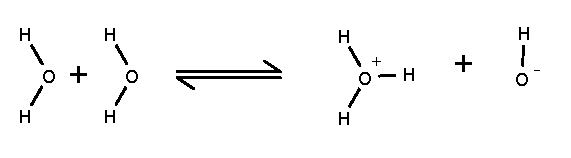
\includegraphics[height=2cm]{autoprotolysis}
\caption{Autoprotolysis of water.}
\label{fig:autoprotolysis}
\end{figure}

The main factor in the reaction is that oxygen is \emph{nucleophilic}, so it attracts electrons. This makes the hydrogen atoms in water
have a positive partial charge and the oxygen atoms a negative partial charge, attracting each other. Due to the nucleophilicity of 
oxygen, a covalent bond can form between them. This bond is formed out of electrons in the outer shell of the oxygen atom not used in bonds so far. Since a hydrogen atom cannot have more than one bond the creation of a new bond is compensated by breaking of the existing hydrogen-oxygen bond.
These reactions are \emph{concerted}, namely they happen together without a stable intermediate configuration. As a result we have reached the state where one oxygen has three covalent bonds to hydrogens and is positively charged,
and the other oxygen bonds to only one hydrogen and is negatively charged. The reaction is reversible: the oxygen, which has lost a hydrogen, can 
pull back one of the hydrogens from the other water.

We now outline the modelling of the reaction in CCB.  % to remind the reader of the basics of CCB. 
We model the hydrogen and oxygen atoms as processes $H$ and $O$ below, where 
$h,o$ are actions representing the bonding capabilities of the atoms and $n,p$ 
represent negative and positive charges respectively. $H',O'$ are process constants.
$$\begin{array}{lll}
H & \bydef & (h;p).H'\\
O & \bydef & (o,o,n).O'
\end{array}$$
We use a general prefixing construct $(s;b).P$ where $s$ is a sequence of actions or executed 
actions, and $b$ is a \emph{weak} action. Sometime the weak action is omitted 
(as in the definition of $O$). Informally, an action in $s$ can take place in any order, 
and $b$ can happen if
all actions in $s$ have already taken place. Once $b$ takes place, it must be accompanied by
undoing immediately one of the actions in $s$ (and thus possibly breaking a bond). We shall later extend
this prefixing operator to permit multiple bonding sites as in $((s;b)\mid \cdots\mid (t;d)).P$.

We use a synchronisation function $\gamma$ which tells us which actions can combine to 
produce bonds between atoms:
$$\begin{array}{llllll}
\gamma(h,o) & = & ho \qquad &
\gamma(n,p) & = & np\\
\gamma(n,h) & = & nh &
\gamma(n,o) & = & no 
\end{array}$$

Each water molecule is a structure consisting of two hydrogen atoms and one oxygen atom 
which are bonded appropriately. 
$$( (h_1[1];p).H'_1 \paral (h_2[2];p).H'_2 \paral (o_1[1],o_2[2],n).O'_1)\setminus\{h_1,h_2,o_1,o_2\}$$
We have used subscripts to name the individual copies of 
atoms and actions. The system of two water molecules in Figure~\ref{fig:autoprotolysis} is represented 
by placing them in parallel and restricting actions $n$ and $p$. This is represented by  
the following process, where restrictions are moved outside using structural congruence laws:
\begin{flalign*}
& ( (h_1[1];p).H'_1 \paral (h_2[2];p).H'_2 \paral (o_1[1],o_2[2],n).O'_1 \paral \\ 
&\paral  (h_3[3];p).H'_3 \paral (h_4[4];p).H'_4  \paral (o_3[3],o_4[4],n).O'_2) 
\setminus\{h_3,h_4,o_3,o_4,h_1,h_2,o_1,o_2,n,p\}
\end{flalign*}
Now actions $n$ and $p$ of different water molecules can combine, representing a transfer of a proton from one atom 
of oxygen to another oxygen. We show below the transfer from $O_2$ to $O_1$, using the \emph{concerted actions} feature of CCB, where the actions to bond are indicated in bold blue and the bond to be broken is in bold red.
\begin{flalign*}
& ( (h_1[1];p).H'_1 \paral (h_2[2];p).H'_2 \paral (o_1[1],o_2[2],\Blue{\bm{n}}).O'_1 \paral 
(\Red{\bm{h_3[3]}};\Blue{\bm{p}}).H'_3 \\
&\paral (h_4[4];p).H'_4  \paral (\Red{\bm{o_3[3]}},o_4[4],n).O'_2) 
\setminus\{h_3,h_4,o_3,o_4,h_1,h_2,o_1,o_2,n,p\}\\
%
&\xrightarrow{\{ np[5], \underline{h_{3}o_{3}}[3]\}} \\
%
&( (h_1[1];p).H'_1 \paral (h_2[2];p).H'_2 \paral (o_1[1],o_2[2],\bm{n[5]}).O'_1 \paral 
(\bm{h_3};\bm{p[5]}).H'_3 \\
&\paral (h_4[4];p).H'_4  \paral (\bm{o_3},o_4[4],n).O'_2) 
\setminus\{h_3,h_4,o_3,o_4,h_1,h_2,o_1,o_2,n,p\}
\end{flalign*}

Since $H_3$ is weakly bonded to $O_1$ and its strong capability 
$h_3$ has become available, the bond $5$ gets promoted to a stronger bond, releasing 
the capability $p$ of $H_3$. This is done by the application of CCB's promotion rule:
\begin{flalign*}
\Rightarrow\; &( (h_1[1];p).H'_1 \paral (h_2[2];p).H'_2 \paral (o_1[1],o_2[2],n[5]).O'_1 \paral 
(h_3[5];p).H'_3 \\
&\paral (h_4[4];p).H'_4  \paral (o_3,o_4[4],n).O'_2) 
\setminus\{h_3,h_4,o_3,o_4,h_1,h_2,o_1,o_2,n,p\}
\end{flalign*}

We have now arrived at the state on the right hand side in Figure~\ref{fig:autoprotolysis}.
Oxygen $O_1$ is blocked, which represents it being fully bonded (and positively charged).
Oxygen  $O_2$ has a free $n$ capability and can abstract any of the hydrogens from $O_1$. 
As a result the process can reverse to its original state or to equivalent states where
different hydrogen atoms are bonded to $O_1$ and $O_2$.

In this paper, we model DNA mismatch repair using the calculus CCB. This builds upon and extends our previous work on the modelling of BER and other biochemical reactions and shows that the mechanisms in CCB are relevant outside its immediate origin. Deoxyribonucleic acid (DNA) carries the essential information for the working of all known organisms. It is composed of two polynucleotide chains. Each nucleotide contains one of the four nucleobases, or simply bases,  adenine (A), cytosine (C), guanine (G), and thymine (T). 
The bases can react with each other as follows: A and T produce a pair A-T, C and G produce a pair C-G,
and other combinations are not normally possible. This property means that each of the two polynucleotide chains of a DNA contains the same biological information, but expressed differently. It also enables DNA replication. 
DNA can split into two chains and then each chain can be completed with the matching bases, so that each new DNA is an identical copy of the original strand. Replication in turn enables the multiplication of cells and growth.

In practice DNA can be imperfect. This could be due either to external factors, such as radiation 
%(the reason why nuclear radition is damaging long-term) 
or internal factors, such as free radicals produced by the body. Another source of DNA errors are problems during replication. For example, it can happen that adenine in one chain faces guanine in the other chain when it should normally be matched by a thymine. Figure~\ref{fig:damages} shows such a mismatch on the right: The combination of the A/G bases is incorrect. Another error is an incorporation of a uracil base (U) in a DNA chain, which would normally not occur in DNA, is shown on the left in Figure~\ref{fig:damages}. A repair mechanism for this error, called Base Excision Repair (BER), was modelled in \cite{10.1007/978-3-319-99498-7_8} using our Calculus of Covalent Bonding (CCB).

\begin{figure}[h!]
  \centering
    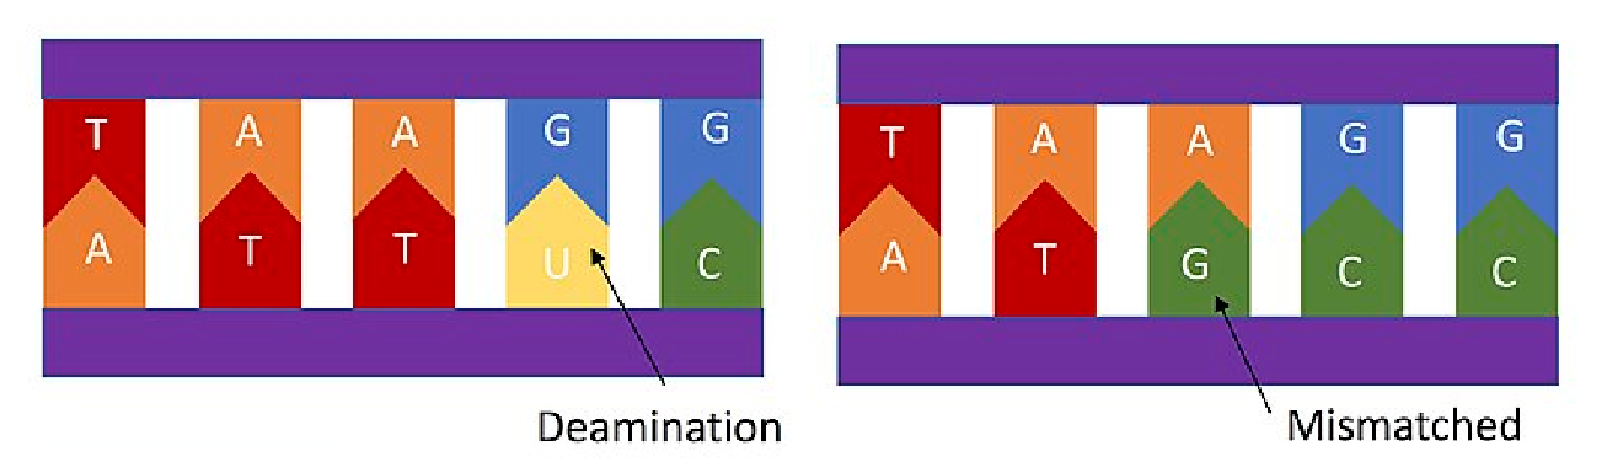
\includegraphics[width=1.0\textwidth]{Types_of_DNA_Damage_part}
  \caption[Two types of DNA damage.]{Two types of DNA damage. The right half shows a DNA mismatch.
  % (the example used here). 
  On the left, the incorporation of a Uracil base is shown.
  %, which was modelled in \cite{10.1007/978-3-319-99498-7_8}. 
  Part of \href{https://commons.wikimedia.org/wiki/File:Types_of_DNA_Damage.jpg}{Image} by Chantelmao, licensed under \href{https://creativecommons.org/licenses/by-sa/4.0/deed.en}{CC-BY-SA-4.0}.}
  \label{fig:damages}
\end{figure}

DNA repair is crucial to maintain the quality of information in organisms. Whilst DNA replication errors are rare (they happen at a rate of about 1 per every 100,000 nucleotides), this translates to a large number of errors given the length of DNA: about 120,000 mistakes every time a human cell divides~\cite{damage}. There are other sources of DNA damage, and also a multitude of repair mechanisms. Here, we focus on a particular type of replication error and its repair. Since incorrect DNA can give rise to cancer and other illnesses and generally to early ageing and death, DNA repair is a crucial part of life and its understanding is an important research topic.

%In this paper, we model DNA mismatch repair using the calculus CCB. This builds upon and extends our previous work on the modelling of BER and other biochemical reactions.
%. The aim of the work is on the one hand to further test and evaluate CCB. On the other hand, it is an extension of the biological modelling done in previous work.

\Comment{
\begin{figure}[h!]
  \centering
    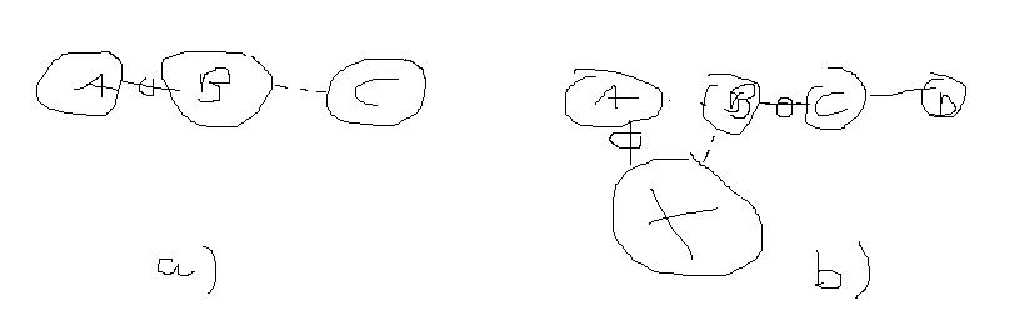
\includegraphics[width=1.0\textwidth]{introexample.ps}
  \caption{The old (left) and new (right) type of concerted actions in CCB. On the left, the formation of a new bond (dashed) triggers breaking of one bond (marked with a circle), whereas on the right two bonds (both marked with a circle) are broken with the formation of one new bond (dashed).}
  \label{fig:introexample}
\end{figure}


\Red{We demonstrate the new operation introduced in this paper informally in Figure~\ref{fig:introexample}. On the left, we see an example of a concerted action as used in CCB so far. Here, the formation of one bond from B to C (dashed) triggers the breaking of one other bond (from A to B, marked with a circle). On the right, the situation is different: There is a chain of objects (A, B, and C, potentially more) and we want another object (X) to move along this chain and break the bonds between the objects at the same time. X is currently bonded to A. For performing a step, it needs to form a new bond to B (dashed), break the old bond to A and break the bond from B to C (both marked with a circle). As we will see, this new mechanism enables the DNA mismatch repair to be modelled in CCB.}

\Red{For modelling such situations, CCB is useful since it enables out-of-causal order reversibility. This is needed to model processes like the one on the rigtht in Figure~\ref{fig:introexample}. Here, a bond to one element (for example A) is needed when the bond to the nexte element (for example B) is formed to avoid losing the connection completely. Only once the new connection is formed, the old one can be released, which is out-of-causal order. A good modelling in a calculus requering causal consistency is not possible.}
}


\section{Related Work}
This work has its origin in two strands of research. One is the simulation of chemical reactions and biological processes. The other is research on process calculi to model computation. These have been merged  to better understand both areas of research. 

In chemistry, speed of reactions and reaction rates have been modelled, with ordinary differential equations (ODEs) being an efficient tool \cite{higham}. Whilst such methods accurately show the dynamic behaviour, it was soon noted that they do not deal with the objects involved. In particular, any properties of the objects, which make reactions possible, are not considered. 
It became even more important when biochemical processes, which do not only involve small molecules, but also macromolecules, cells, and membranes, were modelled. This lack of understanding of the objects was raised in \cite{fontana} and the use of computer science methods like the $\lambda$-calculus was suggested. 

A connection between process calculi and chemistry has been made in \cite{chamjournal}. Here, the Chemical Abstract Machine (CHAM) is introduced as a method to define the semantics of a calculus. As opposed to other semantics for calculi, the algebraic terms (``molecules'') can interact with each other no matter what order they are written in - this is similar to molecules being in a solution. CHAM also introduces membranes to group atoms and rules which simulate heating and cooling of solutions. The actual rules determining the reactions must be defined for a particular CHAM. Therefore, a CHAM can be used to execute processes of arbitrary process calculi. A CHAM can also model actual chemistry depending on the rules used. Starting with Regev et~al.~\cite{regev2000}, process calculi, specifically the $\pi$-calculus, were used to model biochemical systems. There is an analogy between concurrent processes and biological entities in natural systems, and between communication in computer systems and interactions between entities in biological systems. The modelling of biochemical systems is done by representing biological units as processes, and events of binding and unbinding as establishing and breaking a communication, respectively, between processes. The stochastic $\pi$ calculus \cite{PriamiStochasticPi} was used to extend the model to include reaction rates \cite{PriameRegev}. This enables the simulation of the concentrations and of the overall state of the system over time. 

Other work in the area include Bio-PEPA \cite{CiocchettaBiopepa}, which combines a process algebra with timing information and can represent reaction rates. In a Bio-PEPA simulation the entities modelled are species. Every interaction of molecules creates a new species, and there is no tracking of different ``original'' components. The transitions between the entities model the transformations between species. There is no tracking of mechanisms or modelling of the underlying causes. The focus is on the rates and the development of concentrations over time.  

P Systems \cite{psystems} was the first attempt to model membranes and compartments, with objects being able to move in and out of them. A P System contains several membranes, which can be inside one another. For every membrane a set of rules is defined, making P Systems a rule-based system. Objects are located inside membranes, can enter and leave membranes, and membranes can be dissolved. In \cite{CIOBANU2003123} the usage of P Systems for modelling of distributed systems was demonstrated. \cite{CIOBANU2007117} shows that even P systems with minimal parallelism can be universal. An example of a biological application is \cite{10.1007/978-3-540-31837-8_12}, modelling the sodium-potassium pump. 

BioAmbients \cite{RegevBioambients} is based on the Ambient calculus \cite{CARDELLI2000177}, which was originally devised for mobile computing outside the biological context and is an extension of the $\pi$-calculus. Here, similarly to P Systems, processes can be inside compartments.% (and compartments can be in other compartments as well). 
Brane Calculi (``brane'' is short for membrane) \cite{CardelliBraneCalculi}, a family of process calculi, model membranes not only as compartments that define which interactions can happen, but as entities that can be transformed to gain new capabilities. Typical examples are viruses entering cells by interacting with their membranes. The Projective Brane Calculus \cite{ProjectiveBrane} is a variant where interactions are directed outward or inward from a membrane. Other formalims include the Language for Biochemical Systems (LBS) \cite{PlotkinLBS}, the Calculus of Chemical Systems \cite{PlotkinCCS}, and the Biochemical Abstract Machine (BIOCHAM) \cite{biocham}. 

Biochemical reactions are in many cases reversible under certain conditions. The formalisms mentioned do not explicitly model reversibility as undoing of previously performed actions. Instead they use forward actions, which represent undoing of other actions.
%They include potentially actions which are the reverse of other actions, but those reverse actions are independent actions. Logically, they belong together, but this is not modelled. 
The first attempt at the modelling of undoing of forward computation was RCCS~\cite{10.1007/978-3-540-28644-8_19}, a reversible calculus based on CCS. Reversibility is achieved by adding memories to the processes, where a record of past computation is stored. Another reversible calculus based on CCS is CCSK, introduced in \cite{PHILLIPS200770}. It uses keys as a particular form of memory. An extension of CCSK is the Calculus of Covelent Bonding (CCB), which was introduced in~\cite{KU16} and fully defined in~\cite{KU2017}. CCB enables \textit{locally controlled reversibility} by linking forming and breaking of bonds in the syntax of the calculus. CCB has been applied to chemical and biological modelling \cite{10.1007/978-3-319-99498-7_8, Kuhn2020ReversibilityIC}. Reversibility for the $\pi$-calculus was addressed in \cite{10.1007/978-3-642-15375-4_33}. The $\kappa$-calculus \cite{DANOS200469} is based on graph-rewriting. Here, entities (e.g. proteins) are defined as having several sites, which can potentially bind to other entities. The rewrite rules tell that a link can be formed or broken if the sites in the involved entities are in certain states. Reversibility in rule-based systems is discussed in \cite{Aman2020}. 
Petri nets have also been successful in the modelling of biochemical reactions~\cite{10.1007/978-3-540-68894-5_7}. However, traditional Petri nets do not represent reversibility explicitly. Reversibility has only been introduced in Petri nets recently, as can bee seen in \cite{DBLP:conf/rc/PhilippouP18,DBLP:conf/apn/BarylskaGMPPP18,MelgrattiMU20,MelgrattiMPPU20,DBLP:journals/corr/abs-2010-04000}. 


Simple chemical reactions are modelled using CCB, P Systems, and Reversing Petri Nets in~\cite{Kuhn2020ReversibilityIC}. 
%All three formalisms can model the reaction in question, but with some problems being demonstrated. In particular, some reactions emerge from the modelled systems that are not possible in reality. 
An important feature of those formalisms is that they can represent the so-called \emph{out-of-causal order} reversibility~\cite{Irek2012}, where effects can be seemingly undone before their causes are undone, which is important in biological systems. In contrast, most other formalisms for reversible computation, for example RCSS and CCSK, represent \emph{causal-consistent} and \emph{backtracking} reversibility~\cite{DK2007,LPU2020}, where effects can only be undone after all the causes (if any) are undone first.

%
\section{A Calculus of Covalent Bonding}\label{sec:calculus}
%\section{Calculus of Covalent Bonding}\label{sec:calculus}
%
Calculus of Covalent Bonding, or CCB for short, was defined in~\cite{KU2017}. We recall here the main definitions in order to make the paper self-contained. We note, however, that some SOS rules 
are revised and two new SOS rules for concerted actions are added. 
We first introduce some preliminary notions and notations.

Let $\mA$ be the set of (forward) action labels, 
ranged over by $a,b,c,d,e,f$. We partition $\mA$ into the set of \emph{strong actions}, written as
$\mSA$, and the set of \emph{weak actions}, written as $\mWA$. Reverse (or past) action labels are members of
$\underline\mA$, with typical members $\un{a},\un b, \un c,\un d, \un e ,\un f$, and represent 
undoing of actions. The set $\mathcal{P}(\mA \cup \underline\mA)$ is ranged over by $L$.

Let $\Keys$ be an infinite set of {\em communication keys} (or {\em keys} for short)
\cite{PhillipsUlidowski06,Irek2007}, ranged over by $k,l, m,n$. The Cartesian product $\mathcal A \times \Keys$, denoted by $\mAK$,
 represents past actions, which are written as $a[k]$ for $a\in \mA$ and $k\in\Keys$. 
Correspondingly, we have the set $\umAK$ that represents undoing of past actions. Letters $\alpha, \beta$ denote actions which are either from $\mA$ or $\mAK$. It will be 
useful to consider sequences of actions or past actions, namely the elements of $(\mA \cup \mAK)^*$, 
which are ranged over by $s,s'$, and sequences of purely past actions, namely the elements of $\mAK^*$, 
which are ranged over by $t,t'$. The empty sequence is denoted by $\epsilon$. We use $\alpha, s$ and
$s,s'$ to denote a concatenation of elements, which can be strings or single actions.

We shall also use two sets of \emph{auxiliary action} labels, namely the set $(\mA) =\{ (a)\ \mid a\in\mA\}$, and its product with the set of keys, denoted by $(\mA)\Keys$. These labels will be used in the auxiliary rules when defining
the semantics of CCB.

Molecules may have several bonding \emph{sites} and several bonds can be created or dissolved at each bonding site. A site and its potential bonds are modelled via $(s;b)$, where $s$ is a sequence of actions, where actions model bonds, and $b$ is a weak (bond) action. The action $b$ can be omitted, in which case the construct is written as $(s)$. When a molecule has several sites 
$(s;b), \ldots,(s';b')$ we shall write them as $(s;b) \Mid  \ldots \Mid (s';b')$ by using the symbol ``$\paral$'' to indicate that sites bond independently of each other. Such expressions are called \emph{collections of sites}, or just collections, and will be used to define the prefix operator. More formally, a site $\sigma$ is either $(s;b)$ or $(s)$. A collection $\mu$ is either $\sigma$ or $\sigma\Mid\sigma$, and 
$\epsilon$ is the empty collection of sites. We shall denote a collection $\mu$ where all site are fully bonded as $\eta$.


We now define the Calculus of Covalent Bonding. The syntax of CCB is given 
below where $P$ and $Q$ are process terms:

%$$P ::=  S \ \mid \ (s;b).P \ \mid \ P\paral Q \ \mid \ P\restrict L $$
$$P ::=  S \ \mid \ \mu.P \ \mid \ P\paral Q \ \mid \ P\restrict L $$

The set of process identifiers (constants) $\PI$ contains typical elements $S$ and $T$. 
A process identifier $S$ has normally a defining equation $S\bydef P$ where $P$ contains only forward 
actions (and no past actions). There is also a special identifier
 $\Nil$, denoting the deadlocked process, which has no defining equation.

We have a general prefixing operator $\mu.P$. This operator
extends the prefixing operators in \cite{DK2007}, \cite{Irek2012}, and {\cite{KU16,KU2017}. 
If each site of $\mu$ has only one action, then it is the multi-action prefix from \cite{DK2007}.
If the collection $\mu$ has only one site, then it is the general prefixing operator from \cite{KU16,KU2017}. 
If its only site has no weak action, then the prefixing is written as $(s).P$ and is called the
\emph{simple prefix}. 
The simple prefix is the prefixing operator in \cite{Irek2012}. 
One of the actions in $s$ in $(s).P$ may be a weak action from $\mWA$. If $s$ is a sequence that contains   
a single action, then the action is a strong action and the operator 
is the prefixing operator of CCS \cite{Milner1980}.
We omit trailing $\Nil$s so, for example, $(s).\Nil$ is written as $(s)$.
%
% Move this example to somewhere later
%
\Comment{\Stefan{We will only use cases in this paper where processes are of the form $(s).\Nil$. We still have the possibility of 
processes like $(s).(s').\Nil$ in our calculus. This could be used to model protein functions in biological systems, for example 
base excision repair (\cite{Koehler2014}. For this a protein ``walks'' along a strand of DNA and repairs faults which occurred in 
DNA replication. Such a protein could be modelled by having the walk modelled in $s$ and the repair mechanism in $s'$, combining them to a model like $(s).(s').\Nil$.}
}
%
%
The new feature of the operator $(s;b).P$ is the execution of the weak action $b$, which
can happen only after all the actions in $s$ have taken place. Performing $b$ then forces
undoing one of the past actions in $s$ (by the \rulename{concert} rules in Figures~\ref{fig:c1sos}-\ref{fig:xc2sos}).

$P\paral Q$ represents two systems $P$ and $Q$ which can perform actions or reverse actions on
their own, or which can interact with each other according to a communication function
$\gamma$. As in the calculus ACP \cite{ACPBook}, the communication function is a partial function 
$\gamma: \mathcal A \times \mathcal A \rightarrow \mathcal A$ which is commutative and associative. The function
$\gamma$ is used in the operational semantics to define when two processes can interact. Processes 
$P$ and $Q$ in $P\paral Q$ can also perform a pair of concerted actions,
which is the new feature of our calculus.  We also have the ACP-like restriction operator 
$\setminus L$, where $L$ is a set of labels. It prevents actions from taking place and, due to 
the synchronisation algebra used, it also blocks communication. If $\gamma(a,b)=c$ then $a.P$ and $b.Q$
cannot communicate in $(a.P\paral b.Q)\setminus c$.
Note that we do not use here the usual relabelling 
operator $[f]$, where $f: \mA \rightarrow \mA$, which could be easily added.

%
%move this elsewhere?
%
\Comment{
The example in the Introduction and our main example in Section~\ref{sec:bigexample} seem to indicate that only
simple processes of the form $(s;b).\Nil$ are sufficient in the modelling of chemical reactions. 
However, there are examples where a nested prefix $(s;b).(s';b').P$ is useful. 
Consider a base excision repair as in \cite{Koehler2014} where a protein ``walks'' along 
a strand of DNA and repairs faults which occurred in the DNA replication. The walking along a DNA strand 
could be modelled by actions in $s$, and, once a fault is found, the repair mechanism could be modelled
by the actions in $s'$. Another example where the full calculus is useful is a model of long 
standing transactions with compensations in \cite{Irek2012}.
}

The set of \emph{process terms} is ranged over by $P, Q$ and $R$ and is denoted by $\Proc$. 
In the setting of CCB these terms are called \emph{processes}. 
A context $C\hole$ is a process term containing a \emph{hole}, represented by $\hole$. 
Formally, contexts are defined by
the following syntax: $C::= \hole \mid (s;b).C \mid P\paral C \mid C \paral P \mid C\restrict L $.
The term $C[Q]$ denotes the result of filling the hole in the context $C\hole$ with the process $Q$.
We say that $R$ is a \emph{subprocess} of $P$ if $P$ is $C[R]$ for some context $C\hole$.

We define the semantics of our calculus by a labelled transition system,
LTS for short, which is a structure $(St,AL,\rightarrow: \subseteq St \times AL \times St)$
with $St$ the set of states, $AL$ the set of action labels and $\rightarrow: 
\subseteq St \times AL \times St$ the labelled transition relation.
The set of states $St$ is the set $\Proc$. 
%In practice, all our results and examples hold for \emph{consistent} processes, namely processes
%reachable from standard processes.
% (see Definition~\ref{consistent}). 
The action labels are the forward actions $\mAK$, 
the reverse actions $\umAK$ and the \emph{groups of concerted actions} $\mAK \times \umAK \cup 
 \mAK \times \umAK \times \umAK$. 
%
The labelled transition relation is defined by SOS rules (Figures~\ref{fig:fsos}--\ref{fig:sc}) 
and rewrite rules (Figure~\ref{fig:reduction}), where
the rules in Figures~\ref{fig:fsos}--\ref{fig:reversesos}
are influenced by \cite{Irek2007}. 
Note that sequences $s$ and $t$ in Figures~\ref{fig:fsos}--\ref{fig:xc2sos} 
are members of $(\mathcal{A}\cup\mathcal{AK})^*$ and $\mathcal{AK}^*$ respectively.

Next, we recall and explain the SOS rules before returning to 
the rewrite rules. Let $r$ be an SOS rule for an operator $f$ of CCB as in 
Figures~\ref{fig:fsos}--\ref{fig:sc}. 
%Then, $f$ is the operator of $r$ and the elements of $X$ are the arguments of $r$. 
%We write $rules(f)$ for the set of SOS rules for $f$. 
Transitions above the horizontal bar in $r$ are called \emph{premises}. 
The set of premises is written as
$pre(r)$. The transition below the bar in $r$ is the $\emph{conclusion}$ and 
is written as $con(r)$. 

%
\begin{figure}[t] 
\[
\begin{array}{ll}
\Rule
{}
{\std{\Nil}} \quad 
\Rule
{\std{P}}
{\std{S}}
\;\;
S \bydef P
\qquad &
\Rule
{}
{\fresh{m}{\Nil}} \quad
\Rule
{\fresh{m}{P}}
{\fresh{m}{S}}
\;\;
S \bydef P
\\[15pt]
%
\Rule
{\kkey{s}=\emptyset \quad  \std{P}}
{\std{(s;b).P}}
\qquad &
\Rule
{m \notin \kkey{s} \quad \fresh{m}{P}}
{\fresh{m}{(s;b).P}}
\\[15pt]
%
\Rule
{\kkey{s}=\emptyset \quad  \std{\mu.P}}
{\std{((s;b)\Mid \mu).P}}
\qquad &
\Rule
{m \notin \kkey{s} \quad \fresh{m}{\mu.P}}
{\fresh{m}{((s;b)\Mid \mu).P}}
\\[15pt]
%

\qquad &
\Rule
{m \notin \kkey{s} \quad m \neq n \quad \fresh{m}{P}}
{\fresh{m}{(s;b[n]).P}}
\\[15pt]
%
&
\Rule
{m \notin \kkey{s} \quad m \neq n \quad \fresh{m}{\mu.P}}
{\fresh{m}{((s;b[n])\Mid \mu).P}}
\\[15pt]
\Rule
{\std{P} \quad \std{Q}}
{\std{P \paral Q}}\quad 
\Rule
{\std{P}}
{\std{P \setminus L}}
\qquad &
\Rule
{\fresh{m}{P} \quad \fresh{m}{Q}}
{\fresh{m}{P \paral Q}}
\qquad 
\Rule
{\fresh{m}{P}}
{\fresh{m}{P \setminus L}}
\end{array}
\] 
\caption{Predicates $\mathsf{std}$ and $\mathsf{fsh}$.} 
\label{fig:predicates}
\end{figure}
%
%
We use two predicates $\std{P}:\Proc$ and $\fresh{m}{P}:\Keys \times \Proc$ in our SOS rules. 
They are defined in Figure~\ref{fig:predicates}, and they use two auxiliary functions
$\kkey{s}: (\mathcal{A}\cup\mathcal{AK})^* \rightarrow \mathcal{P}(\Keys)$ and
$\keys{P}: \Proc \rightarrow \mathcal{P}(\Keys)$. 
%
The function $\kkey$ is defined as follows:
$\kkey{\epsilon}=\emptyset$, $\kkey{\alpha:s}=\{l\}\cup\kkey{s} \text{ if }\alpha=a[l]$, for 
$a\in \mathcal{A}$ and $l\in \Keys$, and $\kkey{\alpha:s}= \kkey{s} \text{ if }\alpha \in \mathcal{A}$.
%
The function $\keys$ is given by $\keys{\Nil}=\emptyset$, $\keys{S}=\keys{P}$ if $S\bydef P$, 
$\keys{((s;b)\Mid \mu).P}=\kkey{s} \cup \kkey{b} \cup \keys{\mu.P}$, $\keys{P \paral Q}= \keys{P} \cup \keys{Q}$, and $\keys{P \restrict L}=\keys{P}$. Informally $\keys{P}$ associates with each term $P$ the set of its keys. 
A process $P$ is \emph{standard}, written $\std{P}$, if it contains no past actions (hence no keys). 
A key $n$ is \emph{fresh} in $Q$, written $\freshpred{n}(Q)$, if $Q$ contains no past action with the key $n$.
We extend the notion of fresh keys to the sequences of actions and past actions $s$ and $t$, and to sites $\sigma$, 
via the function $\kkey$. Moreover, correspondingly, $\freshpred{n}(\mu)$ if $\freshpred{n}(\sigma)$ for every
site $\sigma$ in $\mu$. 
%Figure~\ref{fig:predicates} defines the predicates by induction over the process terms. 
%We could also have said that $\std{P}$ is true if $\keys{P} = \emptyset$ and that 
%$\fresh{m}{P}$ is true if $i \notin \keys{P}$.

\begin{figure}[t] 
\[
\begin{array}{ll}
\rulename{s}\ 
\Rule
{\fresh{k}{s,s'}}
{(s,a,s';b) \xrightarrow{a[k]}_s (s,a[k],s';b)}
\qquad &
\rulename{c}\
\Rule
{\sigma \xrightarrow{a[k]}_s \sigma'\quad \fresh{k}{\mu}}
{\sigma \paral \mu \xrightarrow{a[k]}_s \sigma' \paral \mu}
%
\\[25pt]
\rulename{act1}\ 
\Rule
{\std{P} \quad \fresh{k}{\mu}\quad \mu \xrightarrow{a[k]}_s \mu'}
{\mu.P \xrightarrow{a[k]}\mu'.P}
\qquad &
\rulename{act2}\
\Rule
{P \xrightarrow{a[k]} P' \quad \fresh{k}{\eta}}
{\eta.P \xrightarrow{a[k]} \eta.P'}
\\[25pt]
%\rom{act3}\ Dec 17
%\Rule
%{\std{P} \quad \fresh{k}{t,t'}}
%{(t,b,t';b').P \xrightarrow{b[k]}(t,b[k],t';b').P}
%\qquad &
%\\[25pt]
\rulename{par}\
\Rule
{P \xrightarrow{a[k]} P'\quad \fresh{k}{Q}}
{P \paral Q \xrightarrow{a[k]} P' \paral Q}
\qquad &
\rulename{com}\
\Rule
{P \xrightarrow{a[k]} P' \quad Q \xrightarrow{d[k]} Q'}
{P \paral Q \xrightarrow{c[k]} P' \paral Q'}
\; (*)
%
\\[25pt]
\rulename{res}\
\Rule
{P \xrightarrow{a[k]} P'}
{P\backslash L \xrightarrow{a[k]} P'\backslash L}
\; a \notin L
\qquad &
\rulename{con}\
\Rule
{P \xrightarrow{a[k]} P'}
{S \xrightarrow{a[k]} P'}
\; S \bydef P
\end{array}
\] 
\caption{Forward SOS rules. The condition (*) is $\gamma(a,d)=c$, 
and $b \in \mathcal{WA}$.} 
\label{fig:fsos}
\end{figure}

\begin{example}
{\rm
We illustrate how processes compute forwards using the new prefixing operator. Initially, we consider processes where collections have single sites only. Consider a standard
process $(a;b).(c) \paral (a,d,c)$ and the communication function $\gamma$ given by $\gamma(a,a)=a$ 
and $\gamma(c,c)=c$. We have
$$(a;b).(c) \paral  (a,d,c) \xrightarrow{a[1]} (a[1];b).(c) \paral  (a[1],d,c)$$
by the SOS rules \rulename{act1} and \rulename{com} from Figure~\ref{fig:fsos}. This is because $(c)$ 
is standard and the key 1 is fresh in $\varepsilon$. The next step of computation involves a communication of
the actions $c$, which we obtain by rules \rulename{act2} and \rulename{com}:
$$(a[1];b).(c) \paral  (a[1],d,c) \xrightarrow{c[2]} (a[1];b).(c[2]) \paral  (a[1],d,c[2])$$
We note that the key 2 is fresh in $a[1]$. Finally, the action $d$ takes place by \rulename{act1} and,
informally, the symmetric version of \rulename{par}.
$$(a[1];b).(c[2]) \paral  (a[1],d,c[2]) \xrightarrow{d[3]} (a[1];b).(c[2]) \paral  (a[1],d[3],c[2])$$
Formally, we use \rulename{par}, the structural congruence rule \rulename{sc} in Figure~\ref{fig:sc}
and the reduction rule \rulename{red1} in Figure~\ref{fig:reduction}.
}
\end{example}

\begin{figure}[t]
\[
\begin{array}{ll}
\rulename{rev s}\ 
\Rule
{\fresh{k}{s,s'}}
{(s,a[k],s';\beta) \xrightarrow{\underline{a}[k]}_s (s,a,s';\beta)}
\qquad &
\rulename{rev c}\
\Rule
{\sigma \xrightarrow{\underline{a}[k]}_s \sigma'\quad \fresh{k}{\mu}}
{\sigma \paral \mu \xrightarrow{\underline{a}[k]}_s \sigma' \paral \mu}
\\[25pt]
%
\rulename{rev act1}\
\Rule
{\std{P} %\quad \fresh{k}{s,s'}
\quad \mu \xrightarrow{\underline{a}[k]}_s \mu' }
{\mu.P \xrightarrow{\underline{a}[k]}\mu'.P}
\quad &
%
% b was previously beta. Since we must apply prom rewrite before we apply any SOS rule, we do not 
% need a rule with a beta.
%
% referees suggested to remove fsh predicates from both act rules. They were there for symmetry reason 
% with the forward rules but are not used in the reverse.
%
\rulename{rev act2}\
\Rule
{P \xrightarrow{\underline{a}[k]} P' %\quad \fresh{k}{t}
}
{\eta.P \xrightarrow{\underline{a}[k]} \eta.P'}
\\[25pt]
% Dec 17
%\rom{rev act3}\
%\Rule
%{\std{P}  \quad \fresh{k}{t,t'} }
%{(t,b[k],t';b').P \xrightarrow{\underline{b}[k]} (t,b,t';b').P'}
%& \\[25pt]
\rulename{rev par}\
\Rule
{P \xrightarrow{\underline{a}[k]} P'\quad \fresh{k}{Q}}
{P \paral Q \xrightarrow{\underline{a}[k]} P' \paral Q}
\quad &
\rulename{rev com}\
\Rule
{P \xrightarrow{\underline{a}[k]} P' \quad Q \xrightarrow{\underline{d}[k]} Q'}
{P \paral Q \xrightarrow{\underline{c}[k]} P' \paral Q'}
\; (*)
%
\\[25pt]
\rulename{rev res}\
\Rule
{P \xrightarrow{\underline{a}[k]} P'}
{P\backslash L \xrightarrow{\underline{a}[k]} P'\backslash L}
\; a \notin L
\quad &
\rulename{rev con}\
\Rule
{P \xrightarrow{\underline{a}[k]} P'}
{P \xrightarrow{\underline{a}[k]} S}
\; S \bydef P'
\end{array}
\]
\caption{Reverse SOS rules. The condition (*) is $\gamma(a,d)=c$, and 
and $b \in \mathcal{WA}$. %Note that $\beta \in \mA \cup \mAK$.
} 
\label{fig:reversesos}
\end{figure}

\begin{figure}[t] 
$$
\begin{array}{l}
\rulename{w}\
\Rule
{\fresh{l}{t}}
{(t;b) \xrightarrow{(b)[l]}_s (t;b[l])} \qquad\qquad
\rulename{cw}\
\Rule
{\sigma \xrightarrow{(b)[l]}_s \sigma'\quad \fresh{l}{\mu}}
{\sigma \paral \mu \xrightarrow{(b)[l]}_s \sigma' \paral \mu}
\\[20pt]
\rulename{aux1}\ 
\Rule{\std{P} \quad \fresh{k}{t}\quad \mu\xrightarrow{(b)[k]}_s \mu'}
{\mu.P \xrightarrow{(b)[k]}\mu'.P}
\qquad
\rulename{aux2}\
\Rule
{P \xrightarrow{(b)[k]} P' \quad \fresh{k}{\eta}}
{\eta.P \xrightarrow{(b)[k]} \eta.P'}
\\[25pt]
\rulename{concert1}\ 
\Rule
{P\xrightarrow{(b)[k]} P'\xrightarrow{\underline{a}[l]}P'' \qquad Q\xrightarrow{\alpha[k]}Q' 
  \quad Q'\xrightarrow{\underline{d}[l]}Q''% %\quad \fresh{k}{Q} 
 }
{P \paral Q\xrightarrow{\{e[k],\underline{f}[l]\}} P'' \paral Q''} (*)\\[25pt]
\rulename{concert2}\ 
\Rule
{U\equiv P \paral Q \quad  P\xrightarrow{(b)[k]}P'\xrightarrow{\underline{a}[l]}P'' 
  \quad Q\xrightarrow{\alpha[k]}Q' 
  \quad R\xrightarrow{\underline{d}[l]}R'% %\quad \fresh{k}{Q} 
 }
{U \paral R\xrightarrow{\{e[k],\underline{f}[l]\}} P'' \paral Q'\paral R'} (*)\\[25pt]
\rulename{concert3}\ 
\Rule
{U\equiv P \paral Q \quad  P\xrightarrow{(b)[k]}P'\xrightarrow{\underline{a}[l]}P'' 
  \quad Q\xrightarrow{\alpha[k]}Q' \xrightarrow{\underline{g}[m]}Q''
  \quad R\xrightarrow{\underline{d}[l],\underline{h}[m]}R'' % %\quad \fresh{k}{Q} 
 }
{U \paral R\xrightarrow{\{e[k],\underline{f}[l]\},\underline{j}[m]} P'' \paral Q''\paral R''} (**)\\[25pt]

\end{array}$$
\caption{SOS rules for concerted actions. The condition (*) is 1. $\alpha$ is $c$ or $(c)$ 
and $\gamma(b,c)=e$ for some $c\in \mathcal{A}$, and 2. $\gamma(a,d)=f$. The condition (**) is (*) additionally with
$\gamma(g,h)=j$.}
\label{fig:c1sos}
\end{figure}


\begin{figure}[t] 
\[
\begin{array}{l}
\rulename{concert2 act}\
\Rule
{P \xrightarrow{\{{a}[k], \underline{h}[l]\}} P' \quad \fresh{k}{t}}
{\eta.P \xrightarrow{\{{a}[k], \underline{h}[l]\}} \eta.P'}\\[25pt]
\rulename{concert3 act}\
\Rule
{P \xrightarrow{\{{a}[k], \underline{h}[l], \underline{j}[m]\}} P' \quad \fresh{k}{t}}
{\eta.P \xrightarrow{\{{a}[k], \underline{h}[l], \underline{j}[m]\}} \eta.P'}\\[25pt]
\rulename{concert2 par}\
\Rule
{P \xrightarrow{\{{a}[k], \underline{h}[l]\}} P'\quad \fresh{k}{Q} \quad \fresh{l}{Q}}
{P \paral Q \xrightarrow{\{{a}[k], \underline{h}[l]\}} P' \paral Q}\\[25pt]
\rulename{concert3 par}\
\Rule
{P \xrightarrow{\{{a}[k], \underline{h}[l], \underline{j}[m]\}} P'\quad \fresh{k}{Q} \quad \fresh{l}{Q}\quad \fresh{m}{Q}}
{P \paral Q \xrightarrow{\{{a}[k], \underline{h}[l], \underline{j}[m]\}} P' \paral Q}\\[25pt]
\rulename{concert2 res}\
\Rule
{P \xrightarrow{\{{a}[k], \underline{h}[l]\}} P'}
{P\backslash L \xrightarrow{\{{a}[k], \underline{h}[l]\}} P'\backslash L}\;\;  a, \underline{h}  \notin L \cup (L)\\[25pt]
\rulename{concert3 res}\
\Rule
{P \xrightarrow{\{{a}[k], \underline{h}[l], \underline{j}[m]\}} P'}
{P\backslash L \xrightarrow{\{{a}[k], \underline{h}[l], \underline{j}[m]\}} P'\backslash L}\;\;  a, \underline{h}, \underline{j}  \notin L \cup (L)
%
\end{array}
\] 
\caption{SOS rules for the prefix, parallel composition and restriction and concerted transitions.
\label{fig:xc2sos} 
}
\end{figure}



\begin{figure}[t] 
\[
\begin{array}{l}
%\rom{sc}\
\Rule
{P \Rightarrow Q \quad Q \tran{\mu} Q' \quad Q' \Rightarrow P'}
{P\tran{\mu} P
'} 
%\quad \mu \in \mAK\cup \umAK \cup \mathcal{C}
%%TODO Moreover, $S\equiv P$ for all $S, P$ 
%%such that $S\bydef P$.
\end{array}
\] 
\caption{Structural congruence rule \rulename{sc} when $\mu\in \mAK \cup (\mAK\times \umAK) \cup  (\mAK\times \umAK\times \umAK))$,
and \rulename{rev sc} when $\mu\in \umAK$.} 
\label{fig:sc}
\end{figure}

\begin{figure}[t] 
\[
\begin{array}{lll}
\rulename{red1}: & P\Par Q \Rightarrow Q\Par P& 
\\[5pt]
\rulename{red2}: & P\Par (Q\Par R) \Rightarrow (P\Par Q)\Par R &
\\[5pt]
\rulename{red3}: & (P\Par Q)\Par R \Rightarrow P\Par (Q\Par R) & 
\\[5pt]
\rulename{red4}: & P\Par \Nil \Rightarrow P & 
\\[5pt]
\rulename{red5}: & (P\paral Q)\backslash L \Rightarrow P\backslash L \paral Q & \mbox{ if fn(Q)} \cap L = \emptyset
\\[5pt]
\rulename{red6}: & P\backslash L \paral Q \Rightarrow (P\paral Q)\backslash L & \mbox{ if fn(Q)} \cap L = \emptyset
\\[5pt]
\rulename{prom}: & (s,a,s';b[k]).P \Rightarrow (s,a[k],s';b).P & \mbox{ if } a \in \mathcal{SA}, b \in \mathcal{WA} 
\\[5pt]
\rulename{move-r}: & (s,a,s',b[k],s'').P \Rightarrow (s,a[k],s',b,s'').P & \mbox{ if } a \in \mathcal{SA}, b \in \mathcal{WA}
\\[5pt]
\rulename{move-l}: & (s,b[k],s',a,s'').P \Rightarrow (s,b,s',a[k],s'').P & \mbox{ if } a \in \mathcal{SA}, b \in \mathcal{WA}
\end{array}
\] 
\caption{Reduction rules. Sequences $s, s', s''$ are members of $(\mathcal{A} \cup \mathcal{AK})^{*}$.} 
\label{fig:reduction}
\end{figure}

The next example illustrates how some of the reverse SOS rules work. We also consider here processes with collections that consist of single sites. 
\begin{example}
{\rm 
Consider $(a[1],b).(c).S$ where $S\bydef (a,b).(c).S$. We have 
$$(a[1],b).(c).S \xrightarrow{\underline{a}[1]} (a,b).(c).S$$ by \rulename{rev act1} since $(c).S$ is standard.
Since $(a,b).(c).S$ is the definition of $S$ we obtain by rule \rulename{rev con} $(a[1],b).(c).S \xrightarrow{\underline{a}[1]} S$.
}
\end{example}

Figures \ref{fig:c1sos}--\ref{fig:xc2sos} contain the SOS rules that define the new concerted actions transitions. 
The main rules are the \rulename{concert} rules in Figure~\ref{fig:c1sos} that define when a pair or a triple 
of concerted action take place. 
We also have four auxiliary rules \rulename{w}, \rulename{cw}, \rulename{aux1} and \rulename{aux2} which 
define only an auxiliary action transition relation needed in the \rulename{concert} rules.
Note that transitions in \rulename{aux1} and \rulename{aux2} use the auxiliary labels $(b)[k]$ 
for all $b \in \mWA$ and $k \in \Keys$. Also note that the three \rulename{concert} rules use \emph{lookahead} \cite{Uli92}.



The rules \rulename{concert par} in Figure~\ref{fig:xc2sos} require that $k$ is fresh in $Q$,
correspondingly as in \rulename{par}. Moreover, we need to ensure that when we reverse $h$ with the key $l$
in $P$ we do not leave out any actions with the key $l$ in $Q$ which make up a multi-action 
communication with the key $l$. Hence, we also include the premise $\fresh{l}{Q}$ in \rulename{concert par} rules. Correspondingly for the key $m$ in $Q$.
The two rules \rulename{concert act} require, correspondingly as \rulename{act}, that $k$ is fresh in $t$.
Our operational semantics guarantees that if a standard process evolves to $(t;b).P$, where all actions in $t$ are fully executed, and
$P$ reverses an action with the key $l$, then $l$ is fresh in $t$. Hence, we do not include $\fresh{l}{t}$
in the premises of the \rulename{concert act} rules.
%
Next, we illustrate how concerted actions transitions work.

\begin{example}\label{ex:examp1}
{\rm Consider the process $(a;b) \paral a \paral b$ with $\gamma(a,a)=c$ and $\gamma(b,d)=f$. After the
initial synchronisation of actions $a$, which produces the transition $c[1]$, we can bond weak $b$ with strong $d$ producing $f$, and at the same time break the $c$ bond. This is represented by a transition
with a pair of concerted actions:
$$(a[1];b) \paral a[1] \paral  b \xrightarrow{\{d[2], \underline{c}[1]\}} 
  (a;b[2])\paral a \paral b[2]$$
The transition is derived by rule \rulename{concert1} in Figure~\ref{fig:c1sos}
 since $(a[1];b) \xrightarrow{(b)[2]} (a[1];b[2]) \xrightarrow{\underline{a}[1]} (a;b[2])$ by \rulename{aux1} and \rulename{rev act1}, 
and since $a[1] \paral b \xrightarrow{b[2]} a[1] \paral b[2] \xrightarrow{\underline{a}[1]} a \paral b[2]$
by \rulename{par} and \rulename{rev par}.}
\end{example}
%
The next example illustrates a creation of a bond between weak actions.
\begin{example}\label{ex:examp2}
{\rm Consider $(a[1];b)\paral (a[1];b)\paral e$ with $\gamma(a,a)=c$ and $\gamma(b,b)=d$. Recall that actions $b$ here are weak.
We have the following pair of concerted actions derived by \rulename{concert1}, where the bond created and the bond broken are between the same two processes:
 $$(a[1];b)\paral (a[1];b)\paral e  \xrightarrow{\{d[2], \underline{c}[1]\}} 
(a;b[2])\paral (a;b[2])\paral e. $$}
\end{example}

There are situations where creation of a bond between two processes with weak actions requires breaking of bonds with other processes. Such transitions cannot be derived by \rulename{concert1}, so we use other concert rules in Figure~\ref{fig:c1sos}.


\begin{example}\label{ex:examp3}
{\rm Consider $(a[1];b)\paral (e[2];b)\paral (a[1],e[2])$ with $\gamma(a,a)=c$, $\gamma(b,b)=d$, and
$\gamma(e,e)=h$.
The process cannot perform any concerted actions by \rulename{concert1}: Although $(a[1];b)  \xrightarrow{(b)[l]} 
\xrightarrow{\underline{a}[1]} (a;b[l])$, for any $l$ different from 1 and 2, but
$(e[2];b)\paral (a[1],e[2])$  cannot perform the auxiliary $(b[l])$
transition since there are no SOS rules for parallel composition and auxiliary actions $(b)$. This forces us
to treat $(a[1];b)$ and $ (e[2];b)$ as $P$ and $Q$ in \rulename{concert1}, respectively, and we notice that
we cannot undo a communication on $a$ or $e$. However, this is precisely what \rulename{concert2} allows, so we have these two concerted transitions:
$$
(a[1];b)\paral (e[2];b)\paral (a[1],e[2])  \xrightarrow{\{d[3], \underline{c}[1]\}} 
(a;b[3])\paral (e[2];b[3])\paral (a,e[2])
$$ 
$$
(a[1];b)\paral (e[2];b)\paral (a[1],e[2])  \xrightarrow{\{d[3], \underline{h}[2]\}} 
(a[1];b[3])\paral (e;b[3])\paral (a[1],e)
$$ 
We notice that, following the first transition, the $h[2]$ bond can be broken, and correspondingly the $c[1]$ bond can be broken after the second transition. Since creation and breaking of such bonds is almost instantaneous, we need a new concert rule that captures such cascade of reactions. Using \rulename{concert3} we derive the following:
$$
(a[1];b)\paral (e[2];b)\paral (a[1],e[2])  \xrightarrow{\{d[3], \underline{c}[1], \underline{h}[2]\}} 
(a;b[3])\paral (e;b[3])\paral (a,e)
$$ 
Here, the bond $d$ is created which results in two other bonds being broken.  }
\end{example}

Overall, the transitions in Figures~\ref{fig:fsos}--\ref{fig:xc2sos} are labelled with $a[k] \in \mAK$, or with 
$\underline{c}[l] \in \umAK$, or with concerted actions $(a[k], \underline{c}[l])$  or $(a[k], \underline{c}[l], \underline{e}[m])$.
%\} \in \mathcal{C}$.

We also have the usual structural congruence rules 
\rulename{sc} and \rulename{rev sc} in Figure~\ref{fig:sc}, 
which potentially combine reductions (defined below) with transitions.

Next, we introduce our reduction relation which is given by the reduction (rewrite) rules 
in Figure~\ref{fig:reduction}. The reduction relation is needed to define {\em promotion} 
of actions. First we define the function $\mathsf{fn}$ for {\em free names} of processes.

\begin{definition} \normalfont 
The function $\mathsf{fn}: \Proc \rightarrow \mathcal{P}(\Keys)$ is given as follows: 
$\mathsf{fn}(\Nil) = \emptyset$,
$\mathsf{fn}(S)=\mathsf{fn}(P) \text{ if }  S\bydef P$, $\mathsf{fn}((\alpha : s;b).P)=\{\alpha\} \cup 
\mathsf{fn}((s;b).P)$, $\mathsf{fn}((a;b).P)=\{a,b\} \cup \mathsf{fn}(P) $, $\mathsf{fn}(P\paral Q)=\mathsf{fn}(P) \cup \mathsf{fn}(Q)$, and $\mathsf{fn}(P \restrict L)=\mathsf{fn}(P) \restrict L$.
\end{definition}

\noindent
The reduction rules have names such as, for example, \rulename{red} and we write 
\rulename{red}: $P \Rightarrow Q$
to indicate that the reduction rule $P \Rightarrow Q$ is called \rulename{red}. 
The process $P$ in the rule
$P\Rightarrow Q$ is called a \emph{redex}, and the process $Q$ is called a \emph{contractum}. 
A reduction rule $P\Rightarrow Q$ can be seen as a prescription 
for deriving rewrites $C[P] \Rightarrow C[Q]$ for arbitrary context $C[\ ]$. 
A $P$ redex may be replaced by its contractum $Q$ in an arbitrary context 
$C[\ ]$ giving rise to a reduction step: $C[P] \Rightarrow C[Q]$.

\begin{definition} \normalfont The reduction relation $\Rightarrow$ is the smallest reflexive and 
transitive relation on CCB processes that is preserved by all contexts, and that satisfies the rules 
in Figure~\ref{fig:reduction}.
\end{definition}
Note that we do not want $\Rightarrow$ to be symmetric as we wish to apply \rulename{prom} only 
from left to right. 

The rewrite rules in Figure~\ref{fig:reduction} include 
\rulename{prom}, \rulename{move-r}, and \rulename{move-l} which  
promote weak bonds (here $b$) to strong bonds (here $a$).
The rule \rulename{prom} applies to the full version of our prefix operator (with the ; construct), and
\rulename{move-r} and \rulename{move-l} apply only to the simple prefix.
These three rules are here to model what happens in chemical systems: a bond on a weak action is 
temporary and as soon as there is a strong action that can accommodate that bond (as the result
of concerted actions) the bond establishes itself on the strong action thus releasing the weak action.
In order to align the use of these three rules to what happens in chemical reactions, we insist
that they are used as soon as they becomes applicable: this is made 
precise in Definition~\ref{LTS}.
We could have used the idea of ordering on SOS rules and rewrite rules \cite{irek2002,mousavi}
to specify that the rewrite rules \rulename{prom}, \rulename{move-r} and \rulename{move-r} are higher 
in the ordering than all SOS rules and the remaining rewrite rules, implying that they should 
be applied first when deriving transitions. Alternatively, we could have tried to 
employ some of the techniques presented in \cite{Cleaveland2001711} to define our transition relation.
This would require the use of negative information in the premisses, and the definitions in the style
as those in \cite{irek2002,mousavi}.  However, since we combine SOS rules
with rewrite rules, we opted for a directly defined transition relation.

We now define the transition relation for the labelled transition system for CCB.
Recall that the states of the LTS are processes in $\Proc$ and the labels are members of $\mA$,
$\mAK$, $\aAK$ and the concerted actions labels in $\mAK \times \umAK$
or $\mAK \times \umAK \times \umAK$. First, the transition relation on collections sites, $\rightarrow_s$, 
is defined as the smallest relation derived by the rules \rulename{s}, \rulename{c},  \rulename{rev s}, \rulename{rev c},   
\rulename{w}, and \rulename{cw} in Figures~\ref{fig:fsos}--\ref{fig:c1sos}.   
%
Let $d:\Proc \rightarrow \mathbb{N}$ be the operator depth function defined by 
$d(P)=0$ if $P$ is a constant, and $d(f(P_1,\ldots,P_n))=1+max\{d(P_i)\vert 1 \leq i \leq n\}$ 
otherwise, where $f$ is an operator of CCB. The transition relation is given as follows:
%
%
\begin{definition}\label{LTS} \normalfont
We associate to $\Proc$ and $\mAK \cup \umAK \cup \aAK \cup (\mAK \times \umAK) 
\cup (\mAK \times \umAK\times \umAK) $
a transition relation
$\rightarrow$ given by $ \bigcup_{l<\omega} \rightarrow^l$, where transition relations
$\rightarrow^l \subseteq \Proc \times \mAK \cup \umAK \cup \aAK \cup (\mAK \times \umAK) \times 
 (\mAK \times \umAK\times \umAK) \Proc$
are as follows, with $b\in \mAK$ and $\mu \in \mAK \cup \umAK \cup (\mAK \times \umAK)
\cup (\mAK \times \umAK\times \umAK) $:

\begin{enumerate}
\item
$P \xrightarrow{(b)[k]} P' \in \rightarrow^l$ if $d(P)=l$,
$P \xrightarrow{(b)[k]} P'= \rho(con(r))$, where $r$ is either \rulename{aux1} or \rulename{aux2},
and each premise in $pre(r)$ is a valid transition in $\bigcup_{k<l} \rightarrow^k$, a valid transition $\rightarrow_s$, 
 or a valid predicate.

\item $P \tran{\mu} P'\in \rightarrow^l$ if $d(P)=l$, $P\Rightarrow Q$, for some $Q$ such that $Q$
does not contain any \rulename{prom}, \rulename{move-r} and \rulename{move-l} redex,  $Q \tran{\mu} Q'= con(r)$,
for some rule $r$ where each member of $pre(r)$ is either a valid transition
in $ \bigcup_{k<l} \rightarrow^k$, a valid transition $\rightarrow_s$, a valid rewrite or a valid predicate, and $Q'\Rightarrow P'$.

\end{enumerate}

\end{definition}


The first part of the definition specifies the auxiliary transitions using rules \rulename{aux1} and 
\rulename{aux2}. The second
part tells us how to use the remaining rules to define transitions. If $P$ has no \rulename{prom}, 
\rulename{move-r} and \rulename{move-l} redex, then we apply our rules in a standard way. Otherwise, we are 
required to reduce $P$ to $Q$ with \rulename{prom}, \rulename{move-r} and \rulename{move-l} first, 
then we define a transition of $Q$ to $Q'$
in a standard way, and finally we reduce $Q'$ to $P'$ (if needed). This implies that 
if $P$ has a \rulename{prom}, \rulename{move-r} or \rulename{move-l} redex, then we must use one 
of the structural congruence rules in Figure \ref{fig:sc}. 
And, if we use any of these rules, then the reduced process $Q$ must no longer have any 
\rulename{prom}, \rulename{move-r} and \rulename{move-l} redex. 
%A different way to define our transition 
%could be to employ some of the techniques suggested in \cite{Cleaveland2001711}
%that employ SOS rules with predicates. This would require the use of negative information in the premisses, 
%so we opted for the alternative approach which is based on the orderings on SOS rules and rewrite rules. 


\Comment{
\Stefan{Our approach for prioritising transitions is different from approaches using predicates in the premises of the SOS rules, as 

suggested for example in \cite{Cleaveland2001711}. In our case we decided for a different approach since we need to prioritise rewrite rules as well as SOS rules.}
}
The next example illustrates the application of the promotion rewrite rule.
\begin{example}\label{example4}
{\rm The transition 
$(a[1];b) \paral a[1] \paral  b \xrightarrow{\{d[2], \underline{c}[1]\}} (a;b[2])\paral a \paral b[2]$ 
from Example \ref{ex:examp1} cannot be followed by a communication of actions $a$ because there
is a \rulename{prom} redex $(a;b[2])$ in $(a;b[2])\paral a \paral b[2]$. The rewrite of this redex takes 
priority: the bond 2 moves from the weak $b$ to the strong $a$ by \rulename{prom}:
$$(a;b[2])\paral a \paral b[2] \Rightarrow (a[2];b)\paral a \paral b[2] $$
As a result, we can bond on the weak $b$ again and, importantly, the $a[2]$ to $b[2]$ bond is irreversible
as $\gamma(a,b)$ is undefined. Note that reaching
this bond by computing forwards alone is not possible.}
\end{example}

We shall call henceforth the transitions derived by the forward SOS rules as the \emph{forward transitions} 
and, the the transitions derived by the reverse SOS rules as the \emph{reverse transitions}.
Correspondingly, there are the \emph{concerted (action)} transitions. 
\subsection{Properties of CCB}
The current version of CCB is a minor extension of the original CCB from \cite{KU2017}. If our collections have only one site, then both calculi have the same syntax. If we additionally do not define rules for concerted transitions that involve three actions, namely \rulename{concert3}, \rulename{concert3 act}, \rulename{concert3 par}, \rulename{concert3 res},
and do not use the alternative rule \rulename{concert2}, then the transition relations that are associated with both calculi are the same. This means that all the properties that the original CCB posses are also enjoyed by the core of the current calculus.

In particular, we can show, using the same arguments as in \cite{KU2017}, that some this CCB satisfies several classical properties of reversible computation such as, for example, \emph{Well-foundedness}, \emph{Reverse Diamond} and \emph{Forward Diamond} \cite{PHILLIPS200770,LPU2020}. Moreover, if we leave out weak actions (and do not use SOS rules that involve weak actions), then the resulting calculus satisfies the \emph{Causal Consistency} property
~\cite{10.1007/978-3-540-28644-8_19,LPU2020}. This gives confidence that the core of CCB models reversibility correctly. 

The purpose of CCB is however to capture the so called ``out-of-causal order'' behaviour which is so common in biochemical reactions. This is achieved via our concerted actions transitions, which allow us faithful modelling of complex sequences of reactions such as those present in a DNA mismatch repair mechanism. 









%
%\section{Base Excision Repair}
%\label{sec:ber}
%
\subsection{Description of Base Excision Repair}

This is from my thesis

So far we have seen some applications of CCB, which are very close to the original inspiration of the calculus. If the principles behind CCB are of some general relevance, there should be other processes we can model using our calculus. A candidate for these might be biological processes. These are ultimately chemical reactions, but they are often viewed at a much higher level of abstraction then we have done so far. Typically, in such studies atoms would no longer play a r\^{o}le, but proteins and other macromolecules, consisting of thousands or more atoms are considered as entities. Typical examples are pathways, gene regulation, transcription, or DNA repair. One of the mechanisms for DNA repair is \emph{base excision repair} (BER). Specifically, BER is responsible for repairing small damages, where a single base pair in the DNA is not correct. Such damages can be inflicted by processes in the body or various external factors like radiation. Repair of such damages is important to prevent a degradation of the DNA information in the organism. There are various subtypes of BER, and various proteins involved in it. For our purposes, we look at the case that a uracil base has been incorporated in the DNA. Uracil is normally only found in RNA, whereas DNA consists of the four bases adenine (A), cytosine (C), guanine (G), and thymine (T).

Uracil-DNA glycosylase (UNG or UDG) is the protein responsible for removing uracil from DNA and making the position available for insertion of the correct base. The process has been extensively studied\footnote{A good overview is given in \cite{pmid25252105}. We use a highly simplified view here. For example, there is not a single UDG, but a family of UDGs all exhibiting slightly different behaviour.} and modelled in \cite{Koehler2014} and \cite{kappadna}. A description of the process on an abstract level is as follows: UDG can bind to any of the deoxyribose/phosphate groups forming the backbone strands of the DNA. From there it can ``walk'' along the chain to the next deoxyribose/phosphate group (that walk makes it much more likely to find a damage than if UDG would just randomly bind to and get off the DNA strand again). If the base attached to this group is uracil, UDG will bind to it and dissolve the bond from the uracil to the DNA. Uracil can then be released and UDG can either continue the search or get off the DNA strand. The correct base can take the place of the uracil.

\subsection{Modelling BER}

In order to model BER, we need the following components: deoxyribose/phosphate groups, the UDG, the uracil and the four other bases. The other bases will not take part in the reactions, but include them in our model in order to demonstrate the interaction we. The components are the following:
%
$$\begin{array}{lll}
DP & \bydef & (p3,p5,b,d).DP'\\
UDG & \bydef & (h;f).(e).UDG'\\
U & \bydef & (b;e).(u).U'\\
A & \bydef & (b;i).(a).A'\\
T & \bydef & (b;i).(t).T'\\
G & \bydef & (b;i).(g).G'\\
C & \bydef & (b;i).(c).C'\\
\end{array}$$
%
where processes $A$, $T$, $G$, $C$, and $U$ model the bases adenine (A), cytosine (C), guanine (G), thymine (T), and uracil (U) respectively. Process $UDG$ represents the Uracil-DNA glycosylase and $DP$ a deoxyribose/phosphate group. Here $d$, $e$, $i$, and $f$ are weak actions, all other actions, namely $p3$, $p5$, $h$, $b$, $u$, $a$, $t$, $g$, and $c$ are strong.

The synchronisation function for our system is as follows:
%
$$\begin{array}{ l c l l }
\gamma(p3,p5) & = & p & \\
\gamma(b,b) & = & bb &\\
\gamma(a,t) & = & at &  \\
\gamma(g,c) & = & gc & \\
\gamma(h,d) & = & hd & \\
\gamma(f,d) & = & fd & \\
\gamma(e,e) & = & ee & \\
\end{array}$$
%
\begin{figure}[h!]
\psfrag{UDG}{${\mathrm{UDG}}$}
\psfrag{sp1}{${\mathrm{DP_1}}$}
\psfrag{sp2}{${\mathrm{DP_2}}$}
\psfrag{sp3}{${\mathrm{DP_3}}$}
\psfrag{sp4}{${\mathrm{DP_4}}$}
\psfrag{sp5}{${\mathrm{DP_5}}$}
\psfrag{sp6}{${\mathrm{DP_6}}$}
\psfrag{A}{${\mathrm{A}}$}
\psfrag{T}{${\mathrm{T}}$}
\psfrag{C1}{${\mathrm{C_1}}$}
\psfrag{C2}{${\mathrm{C_2}}$}
\psfrag{G1}{${\mathrm{G_1}}$}
\psfrag{G2}{${\mathrm{G_2}}$}
\psfrag{U}{${\mathrm{U}}$}
\psfrag{hd}{$hd$}
\psfrag{fd}{$fd$}
  \centering
    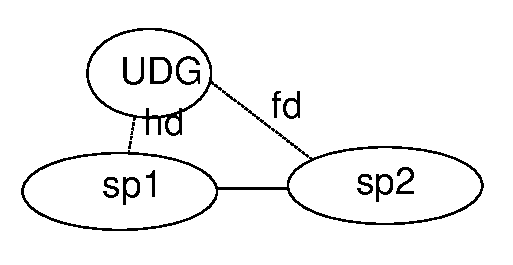
\includegraphics[width=1.0\textwidth]{ber/berintermediate}
  \caption[A $UDG$ unit whilst performing a step along a DNA strand.]{A $UDG$ unit whilst performing a step along a DNA strand. The $hd$ bond is broken together with the new $fd$ being formed.}
  \label{fig:berintermediate}
\end{figure}

We model the deoxyribose/phosphate groups first. This has two ends, normally called 3' and 5', which we model as $p3$ and $p5$ actions respectively. They help us to build the DNA strands. Also, there is a $b$ action, which enables binding of a base. Then we need a possibility for the UDG to bind and to ``walk'': this is enabled by actions $d$, $h$, and $f$, as we will see. UDG is modelled to have the prefix $(h;f)$, which enables the walk, since the strong action $h$ can be bonded to a $DP$ and $f$ can interact with a neighbouring $DP$. This breaks the $hd$ bond, and the $fd$ bond is then promoted to $d$, which gives us the $UDG$ being bonded to the neighbouring $DP$ the same way it was bound before to the other $DP$. Figure~\ref{fig:berintermediate} shows this intermediate situation whilst this step is performed. The five bases ($C$, $G$, $T$, $A$) all have a $b$ action to bind to a $DP$. If $A-T$ respectively $C-G$ are opposite each other they can bind and therefore form a correct base pair in the DNA. Uracil ($U$) is not able to form a base pair in our DNA context. All bases have a weak action in the prefix $(b;x)$. This action $x$ serves for removing the base from the DNA by breaking the $b$ bond. For uracil the action $x$ is $e$, for other bases it is $i$. By this UDG can be specific to uracil. In our model no action interacts with $i$, but of course other proteins not modelled might react with it. Note that $i$ and $e$ actions in the $U$, $A$, $T$, $G$, and $C$ processes cannot happen if the $u, a, t, g$ respctively $c$ actions are done, so $i$ and $e$ are blocked by $u, a, t, g,$ and $c$. Since $u, a, t, g$ and $c$ are used to form the base pairs this means that a correct base pair cannot be removed from the DNA in any case. This models the situation we need for the repair mechanism to work. We have used concerted actions in two instances here: Firstly to enable the UDG walk. This is an instance where backtracking would not work, since we need out-of-causal-order reversibility in this case. We cannot unbond from the old DP first and then choose the next $DP$, but we must hold the old bond until the new bond is formed. Secondly, we use a concerted action to enable the repair mechanism by making a bonding on the repair action break the bond to DP.

In the synchronisation function, we have the interaction of $p3$ and $p5$ to form the strands, the $b$-$b$ interaction for binding the bases, the $h$-$d$ and $f$-$d$ interaction for the ``walk'', the $a$-$t$ and $g$-$c$ interactions for forming the base pairs, and the $e$-$e$ interaction for the repair action.

In order to model a strand of DNA, we restrict ourselves to three base pairs. This means we need six $DP$ processes and six bases. We put two ``correct'' base pairs and one containing a uracil base. An extra $C$ base must be available for replacing $U$. We also use subscripts to distinguish processes where there is more than one instance of the process. The system is modelled in CCB as follows:

$$\begin{array}{l}
(DP_1 \paral DP_2 \paral DP_3 \paral A \paral T \paral G_1 \paral G_2 \paral U \paral C_1 \paral C_2 \paral DP_4 \paral DP_5 \paral DP_6 \paral UDG) \\
\setminus\{p3, p5, d, b, a, t, g, e, u, c, h, f, i\} 
\end{array}$$ 

We leave out the restriction from now on for ease of reading. We number actions using subscripts where there is more than one instance, and set initial bonds as required. We get the following process:
%
\begin{flalign*}
&(p3_1,p5_1[1],d_1,b_1[5]).DP_1' \paral (p3_2[1],p5_2[3],d_2,b_2[4]).DP_2' \paral (p3_3[3],p5_3,d_3,b_3[9]).DP_3' \paral &&\\
&(b_1[5];i_1).(a[6]).A' \paral (b_2[7];i_2).(t[6]).T' \paral (b_3[8];i_3).(g_1).G_1' \paral  ((b_4[9];i_4).(g_2[10]).G_2'  \paral &&\\
&(b_5[4];e_2).(u).U' \paral (b_6[11];i_6).(c_1[10]).C' \paral (b_7;i_7).(c_2).C' \paral (p3_4,p5_4[12],d_4,b_4[7]).DP_4' \paral &&\\ &(p3_5[12],p5_5[13],d_5,b_5[8]).DP_5' \paral (p3_6[13],p5_6,d_6,b_6[11]).DP_6' \paral (h;f).(e_2).UDG'&&
\end{flalign*}
%
\begin{figure}[h!]
\psfrag{UDG}{${\mathrm{UDG}}$}
\psfrag{sp1}{${\mathrm{DP_1}}$}
\psfrag{sp2}{${\mathrm{DP_2}}$}
\psfrag{sp3}{${\mathrm{DP_3}}$}
\psfrag{sp4}{${\mathrm{DP_4}}$}
\psfrag{sp5}{${\mathrm{DP_5}}$}
\psfrag{sp6}{${\mathrm{DP_6}}$}
\psfrag{A}{${\mathrm{A}}$}
\psfrag{T}{${\mathrm{T}}$}
\psfrag{C1}{${\mathrm{C_1}}$}
\psfrag{C2}{${\mathrm{C_2}}$}
\psfrag{G1}{${\mathrm{G_1}}$}
\psfrag{G2}{${\mathrm{G_2}}$}
\psfrag{U}{${\mathrm{U}}$}
\psfrag{1}{${\mathrm{1}}$}
\psfrag{2}{${\mathrm{2}}$}
  \centering
    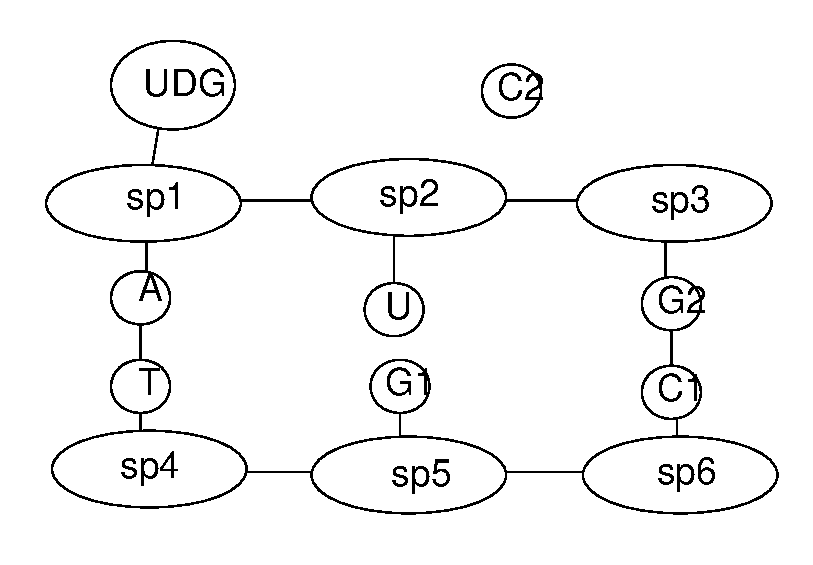
\includegraphics[width=1.0\textwidth]{ber/ber}
  \caption[A three base pair DNA fragment.]{A three base pair DNA fragment, with a uracil instead of a cytosine, and a UDG protein attached.}
  \label{fig:ber}
\end{figure}

Initially $UDG$ bonds to $DP_1$, which in turn is bonded to a correct base pair (note $UDG$ was not bound so far to any other process). The situation is shown in Figure~\ref{fig:ber} and is as follows (the bonds created, news keys and action on which keys were removed are shown in \textbf{bold}):
%
\begin{flalign*}
&\xrightarrow{hd[2]}(p3_1,p5_1[1],d_1\boldsymbol{[2]},b_1[5]).DP_1' \paral (p3_2[1],p5_2[3],d_2,b_2[4]).DP_2' \paral &&\\
&(p3_3[3],p5_3,d_3,b_3[9]).DP_3' \paral
(b_1[5];i_1).(a[6]).A' \paral (b_2[7];i_2).(t[6]).T' \paral (b_3[8];i_3).(g_1).G_1' \paral &&\\
&((b_4[9];i_4).(g_2[10]).G_2'  \paral (b_5[4];e_2).(u).U' \paral (b_6[11];i_6).(c_1[10]).C' \paral (b_7;i_7).(c_2).C' \paral &&\\
&(p3_4,p5_4[12],d_4,b_4[7]).DP_4' \paral (p3_5[12],p5_5[13],d_5,b_5[8]).DP_5' \paral &&\\
&(p3_6[13],p5_6,d_6,b_6[11]).DP_6' \paral (h\boldsymbol{[2]};f).(e_2).UDG'&&
\end{flalign*}
%
The UDG can now randomly ``walk'' along the chain. The $(h;f)$ prefix can appropriately model this, since if the weak $f$ action binds to the neighbour, the bond on $h$ is broken. In our case, action $f$ in $UDG$ can communicate with $d_2$ in $DP_2$. This breaks bond 2 from $h$ in $UDG$ to $d_1$ in $DP_1$, thus having performed a ``step''. We then move key $14$ from $f$ to $h$ (via the \rulename{prom} rule from Figure~\ref{fig:reduction}) and get:
%
\begin{flalign*}
&\xrightarrow{\{fd[14],\underline{hd}[2]\}} \Rightarrow (p3_1,p5_1[1],\boldsymbol{d_1},b_1[5]).DP_1' \paral (p3_2[1],p5_2[3],\boldsymbol{d_2[14]},b_2[4]).DP_2' \paral&&\\
&(p3_3[3],p5_3,d_3,b_3[9]).DP_3' \paral (b_1[5];i_1).(a[6]).A' \paral (b_2[7];i_2).(t[6]).T' \paral (b_3[8];i_3).(g_1).G_1' \paral&&\\
&((b_4[9];i_4).(g_2[10]).G_2'  \paral (b_5[4];e_2).(u).U' \paral (b_6[11];i_6).(c_1[10]).C' \paral (b_7;i_7).(c_2).C' \paral&&\\
&(p3_4,p5_4[12],d_4,b_4[7]).DP_4' \paral (p3_5[12],p5_5[13],d_5,b_5[8]).DP_5' \paral\\ &(p3_6[13],p5_6,d_6,b_6[11]).DP_6' \paral \boldsymbol{(h[14];f)}.(e_2).UDG'&&
\end{flalign*}
%
$UDG$ could now simply continue its walk, or it can interact via its $e$ action with the uracil. Note that other bases expose the $i$ action, so uracil cannot interact with them. The $u$, $a$, $t$, $g$, or $ c$ actions block $e$ or $i$, so correct base pairs are not affected by repairs. In our example $e_2$ on $UDG$ interacts with $e_2$ on $U$, breaking bond 4 between $b_5$ in $UDG$ and $b_2$ in $DP_2$. We have achieved the desired repair, since the uracil is removed from the DNA. We model this by the following transition (we use the rewrite rule again):
%
\begin{flalign*}
&\xrightarrow{\{ee[15],\underline{bb}[4]\}} \Rightarrow (p3_1,p5_1[1],d_1,b_1[5]).DP_1' \paral (p3_2[1],p5_2[3],d_2[14],\boldsymbol{b_2}).DP_2' \paral&&\\
&(p3_3[3],p5_3,d_3,b_3[9]).DP_3' \paral (b_1[5];i_1).(a[6]).A' \paral (b_2[7];i_2).(t[6]).T' \paral (b_3[8];i_3).(g_1).G_1' \paral&&\\
&((b_4[9];i_4).(g_2[10]).G_2'  \paral \boldsymbol{(b_5[15];e_2)}.(u).U' \paral (b_6[11];i_6).(c_1[10]).C' \paral (b_7;i_7).(c_2).C' \paral&&\\
&(p3_4,p5_4[12],d_4,b_4[7]).DP_4' \paral (p3_5[12],p5_5[13],d_5,b_5[8]).DP_5' \paral\\ &(p3_6[13],p5_6,d_6,b_6[11]).DP_6' \paral (h[14];f).(\boldsymbol{e_2[15]}).UDG'&&
\end{flalign*}
%
The floating $C_2$ can now take the place of the $U$ by binding to $DP_2$ and $G_1$. This is represented by the following two transitions:
%
\begin{flalign*}
&\xrightarrow{bb[16]}\xrightarrow{gc[17]}(p3_1,p5_1[1],d_1,b_1[5]).DP_1' \paral (p3_2[1],p5_2[3],d_2[14],\boldsymbol{b_2[16]}).DP_2' \paral&&\\
&(p3_3[3],p5_3,d_3,b_3[9]).DP_3' \paral (b_1[5];i_1).(a[6]).A' \paral (b_2[7];i_2).(t[6]).T' \paral (b_3[8];i_3).(\boldsymbol{g_1[17]}).G_1' \paral&&\\
&((b_4[9];i_4).(g_2[10]).G_2'  \paral (b_5[15];e_2).(u).U' \paral (b_6[11];i_6).(c_1[10]).C' \paral (\boldsymbol{b_7[16]};i_7).(\boldsymbol{c_2[17]}).C' \paral&&\\
&(p3_4,p5_4[12],d_4,b_4[7]).DP_4' \paral (p3_5[12],p5_5[13],d_5,b_5[8]).DP_5' \paral\\ &(p3_6[13],p5_6,d_6,b_6[11]).DP_6' \paral (h[14];f).(e_2[15]).UDG'&&
\end{flalign*}
%
The resulting process is shown in Figure~\ref{fig:ber2}.

\begin{figure}[h!]
\psfrag{UDG}{${\mathrm{UDG}}$}
\psfrag{sp1}{${\mathrm{DP_1}}$}
\psfrag{sp2}{${\mathrm{DP_2}}$}
\psfrag{sp3}{${\mathrm{DP_3}}$}
\psfrag{sp4}{${\mathrm{DP_4}}$}
\psfrag{sp5}{${\mathrm{DP_5}}$}
\psfrag{sp6}{${\mathrm{DP_6}}$}
\psfrag{A}{${\mathrm{A}}$}
\psfrag{T}{${\mathrm{T}}$}
\psfrag{C1}{${\mathrm{C_1}}$}
\psfrag{C2}{${\mathrm{C_2}}$}
\psfrag{G1}{${\mathrm{G_1}}$}
\psfrag{G2}{${\mathrm{G_2}}$}
\psfrag{U}{${\mathrm{U}}$}
\psfrag{1}{${\mathrm{1}}$}
\psfrag{2}{${\mathrm{2}}$}
  \centering
    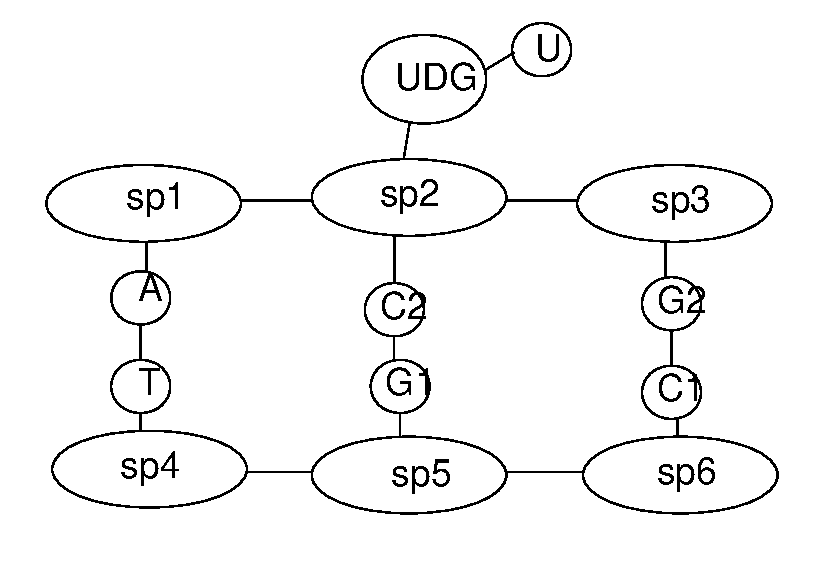
\includegraphics[width=1.0\textwidth]{ber/ber2}
  \caption[The repaired DNA fragment.]{The repaired DNA fragment, with the uracil replaced by a cytosine.}
  \label{fig:ber2}
\end{figure}

If uracil would have been bonded on $u$, the interaction with UDG could not have happened, so the defect is recognized. We now have the uracil broken from the deoxyribose/phosphate group and the $b$ action on the deoxyribose/phosphate group ready to bond to another base. UDG needs to release $U$ and then either to continue its walk or release itself from the DNA. We can again use our new operator for modelling UDG, since this way we achieve that the repair mechanism happens. On the other hand by combining two groups of actions we ``block'' this repair to happen if the desired second bond is there.

A limitation of our modelling is that it allows the UDG during its ``walk'' to bind to any DG group, since there is no restriction which $d$ action is used. In reality of course UDG must continue with the nearest DP group. This is a spatial effect our calculus does not model so far. Similarly, the repair by UDG binding to the $e$ action of a uracil (U) is not dependent on the UDG being next to it, whereas in reality it is. Again this is a spatial effect, which we will discuss in Section~\ref{sec:ccbs}.

We have used the software from Chapter~\ref{sec:simulation} to test the modelling. The desired path is one of the possibilities, which shows that our modelling is adequate in this respect. We also get some undesired reactions: Apart from UDG binding to any DP group during its walk, there is also the possibility that the unused $p5$ action of a $DP$, which is at the end of the DNA strand, interacts with an unused $p3$ from the a DP at the other end of the DNA strand. This is not impossible as a such, but prevented in reality by at least two effects we do not model. One is again the spatial arrangement, the other is the fact that the ends of the DNA are protected by special groups, which we do not model here. They prevent reactions at the DNA ends.

%
\section{DNA Mismatch Repair}\label{sec:dnamimatch}

\subsection{Description of DNA Mismatch Repair}

We now return to the DNA mismatch repair, which we have briefly described in the introduction, and we give a fuller explanation of how it works.
%Such a repair is not possible in the same way as the base excision repair (BER), since any of the two bases could be wrong, so the non-matching  bases do not tell what to do. In contrast, to repair the incorporation of a uracil, clearly the uracil must be removed and replaced. A description of the process on an abstract level is as follows:
If two bases are incorporated into a DNA strand which do not match, namely are not A-T or C-G pairs, this constitutes a defect in the DNA strand. A repair similar to BER is not possible, since it is not clear which of the two bases is correct.
% just from the bases alone - both could be right.
We are looking at a specific way to handle this situation, called Methyl Mismatch Repair (MMR). This is the repair mechanism in bacteria, in particular E.\! coli, for which detailed studies has been done\footnote{Paul L. Modrich, Tomas Lindahl and Aziz Sancar received the Nobel Price in Chemistry 2015 for their work on DNA repair. Modrich's Nobel Lecture about Methyl-directed Mismatch Repair in E. coli and humans \cite{pmid27198632} gives a good overview.}.
The mechanism relies on DNA strands being methylated sometime after their creation. Methylation means the attachment a methyl group (a carbon atom with three hydrogen atoms), in this case to the adenine base A. Specifically, this happens whenever there is a GATC sequence. Since the methylation %(which is done by specific proteins, which we do not model)
happens with a delay after the duplication of a strand, the old strand is methylated and the new strand is not methylated for a short period of time. This enables the removal of the wrong base from the new strand.

The actual repair involves the proteins MutS, MutL, MutH, and UvrD. MutS first binds to the mismatch and then recruits MutL and MutH. MutL can detect the methylated strand and can form a loop in the DNA. In this loop, the newer strand is now outside, whereas the old strand is covered by itself and MutL. Then MutH cleaves the unmethylated strand. This happens in some distance from the mismatch, due to the size of the proteins and the loop in the DNA. UvrD can then detect the cleavage and can move along the strand towards the site of the mismatch. It removes the outer strand when moving along. At the same time, the MutL, MutH, and MutS proteins are released and the loop in the DNA disappears. Finally UvrD moves to a position immediately beyond the mismatch, removing the wrong base together with its neighbours. UvrD then goes off the DNA and leaves the old, and correct, strand to be completed.

\subsection{DNA Mismatch Repair System}

Having briefly introduced all major components that are involved in this mismatch repair mechanism, we now
define them in the syntax of CCB. Our intention is to reuse the components from \cite{10.1007/978-3-319-99498-7_8} as much as possible. Specifically, we reuse the deoxyribose/phosphate groups, and the four bases A, T, C, and G. We will extend those components where needed, but we will keep the original actions. We need the following components for the MMR system: deoxyribose/phosphate groups (DP), the four bases A, T, G, C, the methyl group Me, and the proteins MutS, MutL, MutH, and UvrD. The reused components are as follows:
%
$$\begin{array}{lll}
\DP & \bydef & ((p3,p5;s) \paral (b,d)).\DP'\\
A & \bydef & (b;i).(a,m;r).A'\\
T & \bydef & (b;i).(t;r).T'\\
G & \bydef & (b;i).(g;r).G'\\
C & \bydef & (b;i).(c;r).C'\\
\end{array}$$
%
%where processes $A$, $T$, $G$, and $C$ model the bases adenine (A), cytosine (C), guanine (G), and thymine (T).
Notice that we have added new actions $s$, $m$, and $r$. The action $m$ enables the methylation. It only exists in $A$ since the methylation happens only there. %Also, the actions on DP have been regrouped (but all original actions are still there).
In $\DP$, we now use a collection with two sites. This is necessary to enable breaking of a bond to $p3$ or $p5$, which are on one site, whilst there is still a bond to $b$ on the other site. %The action $d$, which was used by UDG in the modelling of BER is not used here, as we will see. We keep it to have an extension of the previous modelling.

We also need additional components, namely the methyl group Me, and the MutS, MutL, MutH, and UvrD proteins. They are defined as follows:
$$\begin{array}{lll}
\Me & \bydef & (m).(n).\Me' \\
\MutS & \bydef & (k,k).(l).\MutS'\\
\MutL & \bydef & (l).(n).(o).\MutL'\\
\MutH & \bydef & (o).(w).\MutH'\\
\UvrD & \bydef & ((u;r) \paral (v;s)).\UvrD'\\
\end{array}$$
%
%where processes $MutS$, $MutL$, $MutH$, and $UvrD$ model the MutS, MutL, MutH, and UvrD protein respectively.
Here $s$, $i$, and $r$ are weak actions, all other actions, namely $p3$, $p5$, $b$, $d$, $a$, $t$, $g$, $c$, $m$, $n$, $k$, $l$, $o$, $s$, $u$, $v$ and $w$, are strong. Notice that $i$ is not used here, but we keep it to have this model as an extension of the BER model~\cite{10.1007/978-3-319-99498-7_8}. In $\UvrD$, we again use a prefix with two sites.
This will make it possible for $\UvrD$ to break two bonds (one from each site) as it ``moves'' along a DNA strand.


The synchronisation function for our system is as follows:
%
\[\arraycolsep=3.4pt\def\arraystretch{1.0}
\begin{array}{ l c l | l c l | l c l | l c l}
\gamma(p3,p5) & = & p & \gamma(b,b) & = & bb & \gamma(a,t) & = & at &  \gamma(g,c) & = & gc \\
\hline
\gamma(m,m) & = & mm & \gamma(k,a) & = & ka & \gamma(k, g) & = & kg & \gamma(k,c) & = & kc \\
\hline
\gamma(k,t) & = & kt & \gamma(l,l) & = & ll &\gamma(n,n) & = & nn & \gamma(o,o) & = & oo\\
\hline
\gamma(r,r) & = & rr & \gamma(t,u) & = & tu &\gamma(p,s) & = & ps &\gamma(w,s) & = & ws\\
\hline
\gamma(s,p3) & = & sp3 &  \gamma(v,p3) & = & vp3 &\gamma(w,p3) & = & wp3  & \gamma(u,r) & = & ur \\
\hline
\gamma(s,s) & = & ss & \gamma(s,v) & = & sv & \gamma(u,c) &=  & uc &  \\
\end{array}
\]
The deoxyribose/phosphate groups and the bases can combine to form a DNA strand. There can be DNA mismatches in such strands. Note that we do not model how they happen, we just assume a DNA strand as in Figure~\ref{fig:state1} with one DNA mismatch. % and correct pairs otherwise.
The mismatch here is on the $A_2$ and $G_3$ pair.
%, but that is not crucial for our modelling.
The A and G bases cannot bond to each other--it is the case in our model as well as in reality--and this gives the opportunity for the repair. There is a CTAG sequence (respectively a GATC sequence) on the top left (respectively bottom left)
chain of the DNA in Figure~\ref{fig:state1}. This is where the methylation happens. In our case, we have a recently duplicated strand, where the older chain is the upper one ($A_1$ is methylated there) and the newer chain is the lower one (where A is not methylated). The methylation is done by proteins which are not modelled here.
%This is the situation where the MMR can happen.
%
\begin{figure}[h!]
\psfrag{dp1}{$DP_1$}
\psfrag{dp2}{$DP_2$}
\psfrag{dp3}{$DP_3$}
\psfrag{dp4}{$DP_4$}
\psfrag{dp5}{$DP_5$}
\psfrag{dp6}{$DP_6$}
\psfrag{dp7}{$DP_7$}
\psfrag{dp8}{$DP_8$}
\psfrag{dp9}{$DP_9$}
\psfrag{dp10}{$DP_{10}$}
\psfrag{dp11}{$DP_{11}$}
\psfrag{dp12}{$DP_{12}$}
%\psfrag{A1}[cc][][0.8][0]{{$\mathit{A_1}}$}
\psfrag{A1}[cc][][0.8][0]{$A_1$}
\psfrag{A2}[cc][][0.8][0]{$A_2$}
\psfrag{A3}[cc][][0.8][0]{$A_3$}
\psfrag{T1}[cc][][0.8][0]{$T_1$}
\psfrag{T2}[cc][][0.8][0]{$T_2$}
\psfrag{C1}[cc][][0.8][0]{$C_1$}
\psfrag{C2}[cc][][0.8][0]{$C_2$}
\psfrag{C3}[cc][][0.8][0]{$C_3$}
\psfrag{G1}[cc][][0.8][0]{$G_1$}
\psfrag{G2}[cc][][0.8][0]{$G_2$}
\psfrag{G3}[cc][][0.8][0]{$G_3$}
\psfrag{G4}[cc][][0.8][0]{$G_4$}
\psfrag{Me}{${\mathit{Me}}$}
\psfrag{MS}{${\mathit{MutS}}$}
\psfrag{ML}{${\mathit{MutL}}$}
\psfrag{MH}{${\mathit{MutH}}$}
\psfrag{UD}{${\mathit{UvrD}}$}
  \centering
    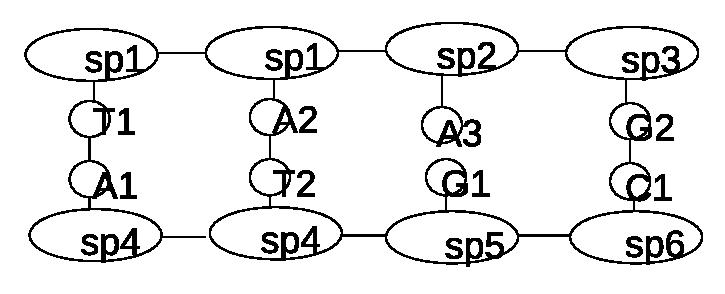
\includegraphics[width=1.0\textwidth]{mmr/state1}
  \caption[A six base pair DNA fragment.]{A six base pair DNA fragment, with a DNA mismatch and methylation of an upper strand. The proteins $\MutL$, $\MutS$, $\MutH$, and $\UvrD$ are not currently bonded to the DNA.}
  \label{fig:state1}
\end{figure}

The system shown in Figure~\ref{fig:state1} is modelled in CCB as follows:
%We can model this similar to what we did before as:
%
$$\begin{array}{l}
(\DP_1 \paral \DP_2 \paral \DP_3 \paral \DP_4 \paral \DP_5 \paral \DP_6 \paral \\
C_1 \paral T_1 \paral A_1 \paral G_1 \paral A_2 \paral C_2 \paral \\
G_2 \paral A_3 \paral T_2 \paral C_3 \paral G_3 \paral G_4 \paral \\
\DP_7 \paral \DP_8 \paral \DP_9 \paral \DP_{10} \paral \DP_{11} \paral \DP_{12} \paral \\
\Me \paral \MutS \paral \MutL \paral \MutH \paral \UvrD) \\
\setminus\{p3, p5, s, i, r, b, b, d, b, a, t, g, c, m, n, k, l, o, s, u, v, w\}
\end{array}$$
%
We leave out the restriction from now on for ease of reading. We mark copies of processes $\DP$ and the bases, and their actions, using subscripts in order to make them unique. Pairs of keys show on which actions the initial bonds have been created. The MMR  system in full detail (but without restriction) is given below.
%
\begin{flalign*}
&((p3_1,p5_1[1];s_1) \paral (b_1[10],d_1)).DP_1' \paral ((p3_2[1],p5_2[2];s_2) \paral (b_2[8],d_2)).DP_2' \paral &&\\
&((p3_3[2],p5_3[3];s_3) \paral (b_3[6],d_3)).DP_3' \paral ((p3_4[3],p5_4[4];s_4) \paral (b_4[9],d_4)).DP_4' \paral &&\\
&((p3_5[4],p5_5[5];s_5) \paral (b_5[7],d_5)).DP_5' \paral ((p3_6[5],p5_6;s_6) \paral (b_6[11],d_6)).DP_6' \paral  &&\\
&(b_{10}[10];i_{10}).(c_1[41];r_{10}).C_1' \paral (b_4[8];i_4).(t_1[23]:r_4).T_1' \paral (b_1[6];i_1).(a_1[24],m_1[40];r_1).A_1' \paral &&\\
& (b_6[9];i_6).(g_1[25];r_6).G_1' \paral (b_2[7];i_2).(a_2,m_2;r_2).A_2' \paral (b_{11}[11];i_{11}).(c_2[27];r_{11}).C_2' \paral &&\\
&(b_7[17];i_7).(g_2[41];r_7).G_2' \paral (b_3[18];i_3).(a_3[23],m_3;r_3).A_3' \paral (b_5[19];i_5).(t_2[24];r_5).T_2' \paral   &&\\
& (b_{12}[20];i_{12}).(c_3[25];r_{12}).C_3'  \paral (b_8[21];i_8).(g_3;r_8).G_3' \paral (b_9[22];i_9).(g_4[27];r_9).G_4' \paral&&\\
&((p3_7,p5_7[12];s_7) \paral (b_7[17],d_7)).DP_7' \paral ((p3_8[12],p5_8[13];s_8) \paral (b_8[18],d_8)).DP_8' \paral &&\\
&((p3_9[13],p5_9[14];s_9) \paral (b_9[19],d_9)).DP_9' \paral ((p3_{10}[14],p5_{10}[15];s_{10}) \paral (b_{10}[20],d_{10})).DP_{10}' \paral  &&\\
&((p3_{11}[15],p5_{11}[16];s_{11}) \paral (b_{11}[21],d_{11})).DP_{11}' \paral ((p3_{12}[16],p5_{12};s_{12}) \paral (b_{12}[22],d_{12})).DP_{12}' \paral  &&\\
&(m[40]).(n).Me'paral (k,k).(l).MutS' \paral (l).(n).(o).MutL' \paral &&\\
&(o).(w).MutH' \paral ((u;r) \paral (v;s)).UvrD'&&
\end{flalign*}
$\DP_1$ is connected to $\DP_2$ via the bond on $p5_1$ and $p3_2$ with the key 1. Similarly, $\DP_1$ is bonded to $C_1$ via the bond on actions $b$ with the key 10. Also, $\Me$ is bonded with $A_1$ on $m$ with the key 40. Correspondingly, there are other initial bonds with appropriate keys in the MMR system as shown in Figure~\ref{fig:state1}. It should be noted that the two processes above show the same system, and so does Figure~\ref{fig:state1}. The two notations above show different levels of detail, with the first only giving the process names and the second their definitions. Figure~\ref{fig:state1} shows the same level of detail as the second process. We do not say how this state emerged and how the bonds were formed.


A mismatch in the DNA section in Figure~\ref{fig:state1} is between $A_2$ and $G_3$.
%: they do not form an A-T or G-C pair as required.
Methylation is on the old upper half of the strand, which means that a methyl group $\Me$ is attached to $A_1$. Note that there is no methyl group on $A_2$. This is because the methylation only happens on CTAG sequences via a specific protein, which we do not model here. %, we just assume the end result.
No bases $A$ are methylated on the new lower half, even if they are part of CTAG sequences, since not enough time has passed at this stage for this to happen.

Before we show the main reactions of the MMR mechanism, we shall shorten the presentation of our MMR system so that the reactions are more easily readable and can be quickly checked.  Since $\DP_1$, $\DP_2$, $\DP_3$, $\DP_4$, $\DP_5$, $\DP_6$, and $\DP_7$, and the bases $C_1$,  $T_1$, $C_2$, $G_2$, $A_3$, and $G_4$  (read from top to bottom and from left to right in Figure~\ref{fig:state1}) never directly participate in the reactions, we will leave them out from now on. The remaining part of the syntax of the MMR system is much smaller:
%
\begin{flalign*}
& (b_1[6];i_1).(a_1[24],m_1[40];r_1).A_1' \paral
(b_6[9];i_6).(g_1[25];r_6).G_1' \paral (b_2[7];i_2).(a_2,m_2;r_2).A_2' \paral  &&\\
& (b_5[19];i_5).(t_2[24];r_5).T_2' \paral
(b_{12}[20];i_{12}).(c_3[25];r_{12}).C_3'  \paral (b_8[21];i_8).(g_3;r_8).G_3' \paral &&\\
&  ((p3_8[12],p5_8[13];s_8) \paral (b_8[18],d_8)).\DP_8' \paral &&\\
&((p3_9[13],p5_9[14];s_9) \paral (b_9[19],d_9)).\DP_9' \paral ((p3_{10}[14],p5_{10}[15];s_{10}) \paral (b_{10}[20],d_{10})).\DP_{10}' \paral  &&\\
&((p3_{11}[15],p5_{11}[16];s_{11}) \paral (b_{11}[21],d_{11})).\DP_{11}' \paral ((p3_{12}[16],p5_{12};s_{12}) \paral (b_{12}[22],d_{12})).\DP_{12}' \paral  &&\\
&(m[40]).(n).\Me'\paral (k,k).(l).\MutS' \paral (l).(n).(o).\MutL' \paral &&\\
&(o).(w).\MutH' \paral ((u;r) \paral (v;s)).\UvrD'&&
\end{flalign*}
Note that leaving out some components results in appearance of  several ``incomplete'' bonds, for example, between
$\DP_8$ and $\DP_7$, which is left out, with the key 12.

\subsection{Reactions in DNA Mismatch Repair}


We now present the main reactions of the MMR system, thus illustrating the benefits of concerted actions transitions.

 We start with the protein $\MutS$ bonding to processes $A_2$ and $G_3$  via the $a_2$ and $g_3$ actions respectively. This is the recognition of the mismatch.
%Note that the $a$ and $g$ actions are not available on matching pairs. So the bonding is not possible if the bases are properly paired, and also not if a Uracil is incorporated into the strand (as in the BER example).
The transitions for creating the two bonds of $\MutS$ with
$A_2$ and $G_3$ are as follows, where first we highlight the participating actions in bold blue font and then we
highlight the actions and keys in bold black font after the bonds are created:

\begin{flalign*}
& (b_1[6];i_1).(a_1[24],m_1[40];r_1).A_1' \paral
(b_6[9];i_6).(g_1[25];r_6).G_1' \paral & & \\
& (b_2[7];i_2).(\Blue{\bm{a_2}},m_2;r_2).A_2' \paral  (b_5[19];i_5).(t_2[24];r_5).T_2' \paral
(b_{12}[20];i_{12}).(c_3[25];r_{12}).C_3'  \paral & & \\
& (b_8[21];i_8).(\Blue{\bm{g_3}};r_8).G_3' \paral  ((p3_8[12],p5_8[13];s_8) \paral (b_8[18],d_8)).\DP_8' \paral &&\\
&((p3_9[13],p5_9[14];s_9) \paral (b_9[19],d_9)).\DP_9' \paral ((p3_{10}[14],p5_{10}[15];s_{10}) \paral (b_{10}[20],d_{10})).\DP_{10}' \paral  &&\\
&((p3_{11}[15],p5_{11}[16];s_{11}) \paral (b_{11}[21],d_{11})).\DP_{11}' \paral ((p3_{12}[16],p5_{12};s_{12}) \paral (b_{12}[22],d_{12})).\DP_{12}' \paral  &&\\
&(m[40]).(n).\Me'\paral (\Blue{\bm{k}},\Blue{\bm{k}}).(l).\MutS' \paral (l).(n).(o).\MutL' \paral &&\\
&(o).(w).\MutH' \paral ((u;r) \paral (v;s)).\UvrD'&&\\
%
&\xxrightarrow{ka[28]} \xxrightarrow{kg[29]} &&\\
%
& (b_1[6];i_1).(a_1[24],m_1[40];r_1).A_1' \paral (b_6[9];i_6).(g_1[25];r_6).G_1' \paral &&\\
&(b_2[7];i_2).(\bm{a_2[28]},m_2;r_2).A_2' \paral  (b_5[19];i_5).(t_2[24];r_5).T_2' \paral (b_{12}[20];i_{12}).(c_3[25];r_{12}).C_3'  \paral &&\\
&(b_8[21];i_8).(\bm{g_3[29]};r_8).G_3' \paral ((p3_8[12],p5_8[13];s_8) \paral (b_8[18],d_8)).\DP_8' \paral &&\\
&((p3_9[13],p5_9[14];s_9) \paral (b_9[19],d_9)).\DP_9' \paral ((p3_{10}[14],p5_{10}[15];s_{10}) \paral (b_{10}[20],d_{10})).\DP_{10}' \paral &&\\
&((p3_{11}[15],p5_{11}[16];s_{11}) \paral (b_{11}[21],d_{11})).\DP_{11}' \paral ((p3_{12}[16],p5_{12};s_{12}) \paral (b_{12}[22],d_{12})).\DP_{12}' \paral  &&\\
&(m[40]).(n).\Me'\paral (\bm{k[28],k[29]}).(\Blue{\bm{l}}).\MutS' \paral (\Blue{\bm{l}}).(n).(o).\MutL' \paral &&\\
&(o).(w).\MutH' \paral ((u;r) \paral (v;s)).\UvrD'&&
\end{flalign*}

Now it is possible for $\MutL$ to bond to $\MutS$ on $l$ with key 30 (see Figure~\ref{fig:state15}). Again, the participating actions $l$ are in bold blue font before the transition and then they are displayed in bold black font:
%
\begin{flalign*}
&\xxrightarrow{ll[30]} (b_1[6];i_1).(a_1[24],m_1[40];r_1).A_1' \paral (b_6[9];i_6).(g_1[25];r_6).G_1' \paral &&\\
&(b_2[7];i_2).(a_2[28],m_2;r_2).A_2' \paral (b_5[19];i_5).(t_2[24];r_5).T_2' \paral  (b_{12}[20];i_{12}).(c_3[25];r_{12}).C_3'  \paral &&\\
&(b_8[21];i_8).(g_3[29];r_8).G_3' \paral ((p3_8[12],p5_8[13];s_8) \paral (b_8[18],d_8)).\DP_8' \paral &&\\
&((p3_9[13],p5_9[14];s_9) \paral (b_9[19],d_9)).\DP_9' \paral ((p3_{10}[14],p5_{10}[15];s_{10}) \paral (b_{10}[20],d_{10})).\DP_{10}' \paral  &&\\
&((p3_{11}[15],p5_{11}[16];s_{11}) \paral (b_{11}[21],d_{11})).\DP_{11}' \paral ((p3_{12}[16],p5_{12};s_{12}) \paral (b_{12}[22],d_{12})).\DP_{12}' \paral &&\\
&(m[40]).(\Blue{\bm{n}}).\Me'\paral (k[28],k[29]).(\bm{l[30]}).\MutS' \paral (\bm{l[30]}).(\Blue{\bm{n}}).(o).\MutL' \paral &&\\
&(o).(w).\MutH' \paral ((u;r) \paral (v;s)).\UvrD'&&
\end{flalign*}

$\MutL$ then bonds with $\Me$ on $n$, which means it detects which of the strands is methylated, and therefore the correct one:
%
\begin{flalign*}
&\xxrightarrow{nn[31]} (b_1[6];i_1).(a_1[24],m_1[40];r_1).A_1' \paral (b_6[9];i_6).(g_1[25];r_6).G_1' \paral &&\\
&(b_2[7];i_2).(a_2[28],m_2;r_2).A_2' \paral (b_5[19];i_5).(t_2[24];r_5).T_2' \paral  (b_{11}[20];i_{11}).(c_3[25];r_{12}).C_3'  \paral&&\\
&(b_8[21];i_8).(g_2[29];r_8).G_3' \paral ((p3_8[12],p5_8[13];s_8) \paral (b_8[18],d_8)).\DP_8' \paral &&\\
&((p3_9[13],p5_9[14];s_9) \paral (b_9[19],d_9)).\DP_9' \paral ((p3_{10}[14],p5_{10}[15];s_{10}) \paral (b_{10}[20],d_{10})).\DP_{10}' \paral &&\\
&((p3_{11}[15],p5_{11}[16];s_{11}) \paral (b_{11}[21],d_{11})).\DP_{11}' \paral ((p3_{12}[16],p5_{12};s_{12}) \paral (b_{12}[22],d_{12})).\DP_{12}' \paral  &&\\
&(m[40]).(\bm{n[31]}).\Me'\paral (k[28],k[29]).(l[30]).\MutS' \paral (l[30]).(\bm{n[31]}).(\Blue{\bm{o}}).\MutL' \paral 
&&\\
&(\Blue{\bm{o}}).(w).\MutH' \paral ((u;r) \paral (v;s)).\UvrD'&&
\end{flalign*}
%
Finally, $\MutL$ recruits $\MutH$.
Henceforth, we shall use bold red font to highlight actions and keys of bonds that will be next broken. Once the bonds are broken, their actions will be shown in bold black font.
%
\begin{flalign*}
&\xxrightarrow{oo[32]} (b_1[6];i_1).(a_1[24],m_1[40];r_1).A_1' \paral (b_6[9];i_6).(g_1[25];r_6).G_1' \paral  &&\\
&(b_2[7];i_2).(a_2[28],m_2;r_2).A_2' \paral (b_5[19];i_5).(t_2[24];r_5).T_2' \paral (b_{12}[20];i_{12}).(c_3[25];r_{12}).C_3'  \paral&&\\
&(b_8[21];i_8).(g_3[29];r_8).G_3' \paral ((p3_8[12],\Red{\bm{p5_8[13]}};\Blue{\bm{s_8}}) \paral (b_8[18],d_8)).\DP_8' \paral &&\\
&((\Red{\bm{p3_9[13]}},p5_9[14];s_9) \paral (b_9[19],d_9)).\DP_9' \paral ((p3_{10}[14],p5_{10}[15];s_{10}) \paral (b_{10}[20],d_{10})).\DP_{10}' \paral &&\\
& ((p3_{11}[15],p5_{11}[16];s_{11}) \paral (b_{11}[21],d_{11})).\DP_{11}' \paral ((p3_{12}[16],p5_{12};s_{12}) \paral (b_{12}[22],d_{12})).\DP_{12}' \paral &&\\
&(m[40]).(n[31]).\Me'\paral (k[28],k[29]).(l[30]).\MutS' \paral (l[30]).(n[31]).(\bm{o[32]}).\MutL' \paral &&\\
&(\bm{o[32]}).(\Blue{\bm{w}}).\MutH' \paral ((u;r) \paral (v;s)).\UvrD'&&
\end{flalign*}
%

The system at this stage is shown in Figure~\ref{fig:state15}. 
%The bond to broken next (between $DP_8$ and $DP_9$) is displayed as a red dashed line, and henceforth we shall use this representation for bonds to be broken.
%
\begin{figure}[h!]
\psfrag{28}[cc][][0.8][0]{$28$}
\psfrag{29}[cc][][0.8][0]{$29$}
\psfrag{30}[cc][][0.8][0]{$30$}
\psfrag{31}[cc][][0.8][0]{$31$}
\psfrag{32}[cc][][0.8][0]{$32$}
\psfrag{dp1}{$DP_1$}
\psfrag{dp2}{$DP_2$}
\psfrag{dp3}{$DP_3$}
\psfrag{dp4}{$DP_4$}
\psfrag{dp5}{$DP_5$}
\psfrag{dp6}{$DP_6$}
\psfrag{dp7}{$DP_7$}
\psfrag{dp8}{$DP_8$}
\psfrag{dp9}{$DP_9$}
\psfrag{dp10}{$DP_{10}$}
\psfrag{dp11}{$DP_{11}$}
\psfrag{dp12}{$DP_{12}$}
%\psfrag{A1}[cc][][0.8][0]{{$\mathit{A_1}}$}
\psfrag{A1}[cc][][0.8][0]{$A_1$}
\psfrag{A2}[cc][][0.8][0]{$A_2$}
\psfrag{A3}[cc][][0.8][0]{$A_3$}
\psfrag{T1}[cc][][0.8][0]{$T_1$}
\psfrag{T2}[cc][][0.8][0]{$T_2$}
\psfrag{C1}[cc][][0.8][0]{$C_1$}
\psfrag{C2}[cc][][0.8][0]{$C_2$}
\psfrag{C3}[cc][][0.8][0]{$C_3$}
\psfrag{G1}[cc][][0.8][0]{$G_1$}
\psfrag{G2}[cc][][0.8][0]{$G_2$}
\psfrag{G3}[cc][][0.8][0]{$G_3$}
\psfrag{G4}[cc][][0.8][0]{$G_4$}
\psfrag{Me}{${\mathit{Me}}$}
\psfrag{MS}{${\mathit{MutS}}$}
\psfrag{ML}{${\mathit{MutL}}$}
\psfrag{MH}{${\mathit{MutH}}$}
\psfrag{UD}{${\mathit{UvrD}}$}
  \centering
    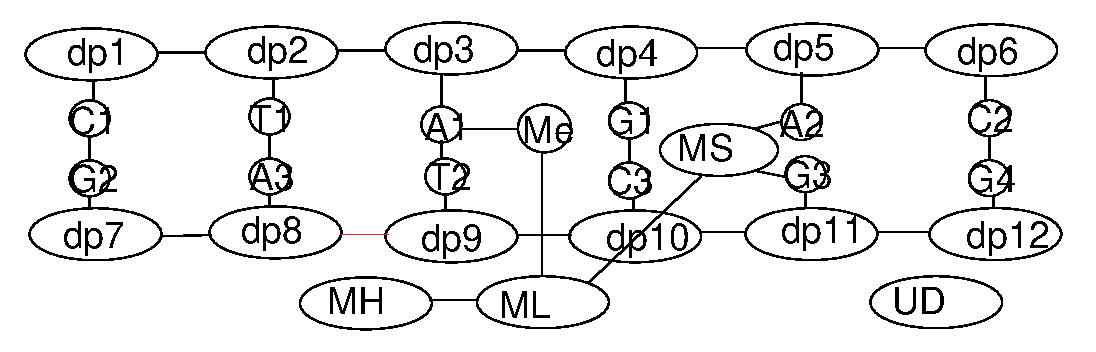
\includegraphics[width=1.0\textwidth]{mmr/state15}
  \caption[A six base pair DNA fragment.]{A six base pair DNA fragment, with a DNA mismatch and methylation of one strand. The proteins $\MutL$, $\MutS$, and  $\MutH$ are bonded to the strand and ready to recruit $\UvrD$, which at this point is not
  involved yet.}
  \label{fig:state15}
\end{figure}

Next, $\MutH$ is ready to cleave the DNA at the right location. This is done by bonding to $\DP_8$ with the key 33 and, at the same time, breaking the bond between $\DP_8$ and $\DP_9$ (with the key 13). These two simultaneous reactions are represented by the following concerted actions transition.

\begin{flalign*}
&\xrightarrow{\{ws[33],\underline{p}[13]\}} (b_1[6];i_1).(a_1[24],m_1[40];r_1).A_1' \paral (b_6[9];i_6).(g_1[25];r_6).G_1' \paral  &&\\
&(b_2[7];i_2).(a_2[28],m_2;r_2).A_2' \paral (b_5[19];i_5).(t_2[24];r_5).T_2' \paral (b_{12}[20];i_{12}).(c_3[25];r_{12}).C_3'  \paral&&\\
&(b_8[21];i_8).(g_3[29];r_8).G_3' \paral ((p3_8[12],\bm{p5_8};\bm{s_8[33]}) \paral (b_8[18],d_8)).DP_8' \paral &&\\
&((\bm{p3_9},p5_9[14];s_9) \paral (b_9[19],d_9)).DP_9' \paral ((p3_{10}[14],p5_{10}[15];s_{10}) \paral (b_{10}[20],d_{10})).DP_{10}' \paral  &&\\
&((p3_{11}[15],p5_{11}[16];s_{11}) \paral (b_{11}[21],d_{11})).DP_{11}' \paral ((p3_{12}[16],p5_{12};s_{12}) \paral (b_{12}[22],d_{12})).DP_{12}' \paral  &&\\
&(m[40]).(n[31]).Me'\paral (k[28],k[29]).(l[30]).MutS' \paral (l[30]).(n[31]).(o[32]).MutL' \paral &&\\
&(o[32]).(\bm{w[33]}).MutH' \paral ((u;r) \paral (v;s)).UvrD'&&
\end{flalign*}
Next, {\em promotion} happens, which moves the bond with the key 33 from a weak action $s_8$ to a strong action $p5_8$ in one of the sites of $\DP_8$:
\begin{flalign*}
&\overset{ \rulename{prom}}\Rightarrow (b_1[6];i_1).(a_1[24],m_1[40];r_1).A_1' \paral (b_6[9];i_6).(g_1[25];r_6).G_1' \paral  &&\\
&(b_2[7];i_2).(a_2[28],m_2;r_2).A_2' \paral (b_5[19];i_5).(t_2[24];r_5).T_2' \paral (b_{12}[20];i_{12}).(c_3[25];r_{10}).C_3'  \paral &&\\
&(b_8[21];i_8).(g_3[29];r_8).G_3' \paral ((p3_8[12],\bm{p5_8[33]};\bm{s_8}) \paral (b_8[18],d_8)).DP_8' \paral &&\\
&((p3_9,\Red{\bm{p5_9[14]}};s_9) \paral (b_9[19],d_9)).DP_9' \paral ((\Red{\bm{p3_{10}[14]}},p5_{10}[15];\Blue{\bm{s_{10}}}) \paral (b_{10}[20],d_{10})).DP_{10}' \paral  &&\\
&((p3_{11}[15],p5_{11}[16];s_{11}) \paral (b_{11}[21],d_{11})).DP_{11}' \paral ((p3_{12}[16],p5_{12};s_{12}) \paral (b_{12}[22],d_{12})).DP_{12}' \paral  &&\\
&(m[40]).(n[31]).Me'\paral (k[28],k[29]).(l[30]).MutS' \paral (l[30]).(n[31]).(o[32]).MutL' \paral &&\\
&(o[32]).({w[33]}).MutH' \paral ((u;r) \paral (\Blue{\bm{v}};s)).UvrD'&&
\end{flalign*}

These two transitions give us the corresponding $\xxrightarrow{\{ws[33],\underline{p}[13]\}}$ by Definition~\ref{LTS}.

Note that $\MutH$ bonding with $\DP_8$ on $s_8$ (key 33) leads to breaking the bond between two deoxyribose/phosphate groups $\DP_8$ and $\DP_9$ (key13). 
%
%Note that execution of $s_8$ on $\DP_8$ leads to breaking a bond between two deoxyribose/phosphate groups. Specifically, bond 33 from $\MutH$ to $DP_8$ via actions $w$ and $s$ is formed and bond 13 between $p5$ in $\DP_8$ and $p3$ in  $\DP_9$ is broken. %We use concerted actions and rewriting for this.
%
The situation after this step is shown in Figure~\ref{fig:state2}, where the new bond (key 33) is shown as a blue line. The broken bond (key 13) is indicated by a red dotted line, and henceforth, we shall use this representation for broken bonds. Such dotted lines will be left out in subsequent figures to indicate that the relevant bonds no longer exist.  This has now the right DNA strand cleaved.

\begin{figure}[h!]
\psfrag{13}[cc][][0.8][0]{$13$}
\psfrag{33}[cc][][0.8][0]{$33$}
\psfrag{dp1}{$DP_1$}
\psfrag{dp2}{$DP_2$}
\psfrag{dp3}{$DP_3$}
\psfrag{dp4}{$DP_4$}
\psfrag{dp5}{$DP_5$}
\psfrag{dp6}{$DP_6$}
\psfrag{dp7}{$DP_7$}
\psfrag{dp8}{$DP_8$}
\psfrag{dp9}{$DP_9$}
\psfrag{dp10}{$DP_{10}$}
\psfrag{dp11}{$DP_{11}$}
\psfrag{dp12}{$DP_{12}$}
\psfrag{A1}[cc][][0.8][0]{$A_1$}
\psfrag{A2}[cc][][0.8][0]{$A_2$}
\psfrag{A3}[cc][][0.8][0]{$A_3$}
\psfrag{T1}[cc][][0.8][0]{$T_1$}
\psfrag{T2}[cc][][0.8][0]{$T_2$}
\psfrag{C1}[cc][][0.8][0]{$C_1$}
\psfrag{C2}[cc][][0.8][0]{$C_2$}
\psfrag{C3}[cc][][0.8][0]{$C_3$}
\psfrag{G1}[cc][][0.8][0]{$G_1$}
\psfrag{G2}[cc][][0.8][0]{$G_2$}
\psfrag{G3}[cc][][0.8][0]{$G_3$}
\psfrag{G4}[cc][][0.8][0]{$G_4$}
\psfrag{Me}{${\mathit{Me}}$}
\psfrag{MS}{${\mathit{MutS}}$}
\psfrag{ML}{${\mathit{MutL}}$}
\psfrag{MH}{${\mathit{MutH}}$}
\psfrag{UD}{${\mathit{UvrD}}$}
  \centering
    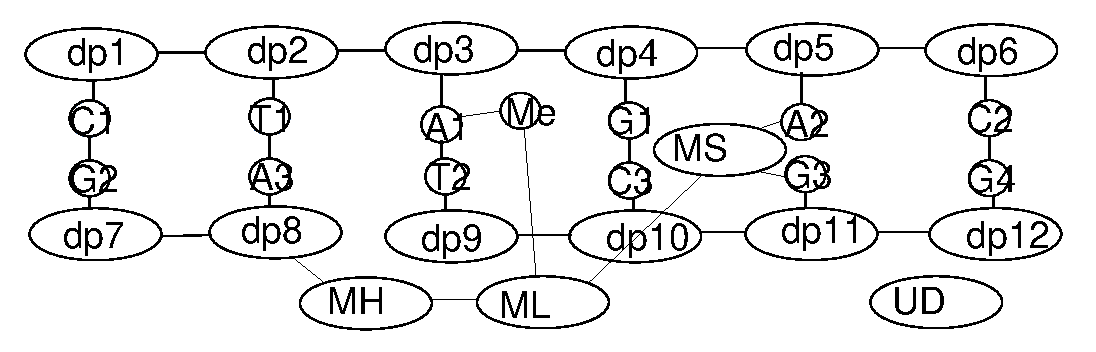
\includegraphics[width=1.0\textwidth]{mmr/state2}
  \caption[A six base pair DNA fragment.]{%A six base pair DNA fragment, with a DNA mismatch and methylation of one strand.
  The mismatch has been detected by $\MutS$, and $\MutH$ and $\MutL$ have been recruited. $\MutL$ has detected the methylation, and $\MutH$ has cleaved the strand containing the wrong base by bonding to $DP_8$ (blue line) and thus breaking the bond between $DP_8$ and $DP_9$ (red dotted line).}
  \label{fig:state2}
\end{figure}

Next, the protein $\UvrD$ gets involved in the repair. It uses the cleavage to remove pairs of deoxyribose/phosphate groups and bases.
Firstly, $\UvrD$ bonds to $\DP_{10}$ (key 34) and thus breaks the bond between $\DP_{10}$ and its left neighbour
$\DP_9$ (key 14). Then the bond 34 is promoted from weak $s_{10}$ to strong $p3_{10}$:

\begin{flalign*}
%&\xrightarrow{\{sv[34],\underline{p}[14]\}}  \overset{ \rulename{prom}}\Rightarrow  
&\xxrightarrow{\{sv[34],\underline{p}[14]\}}  
(b_1[6];i_1).(\Red{\bm{a_1[24]}},m_1[40];r_1).A_1' \paral  (b_6[9];i_6).(g_1[25];r_6).G_1' \paral &&\\
&(b_2[7];i_2).(a_2[28],m_2;r_2).A_2' \paral (b_5[19];i_5).(\Red{\bm{t_2[24]}};\Blue{\bm{r_5}}).T_2' \paral (b_{12}[20];i_{12}).(c_3[25];r_{12}).C_3'  \paral&&\\
&(b_8[21];i_8).(g_3[29];r_8).G_3' \paral ((p3_8[12],p5_8[33];s_8) \paral (b_8[18],d_8)).\DP_8' \paral &&\\
&((p3_9,\bm{p5_9};s_9) \paral (b_9[19],d_9)).\DP_9' \paral ((\bm{p3_{10}[34]},p5_{10}[15];\bm{s_{10}}) \paral (b_{10}[20],d_{10})).\DP_{10}' \paral  &&\\
&((p3_{11}[15],p5_{11}[16];s_{11}) \paral (b_{11}[21],d_{11})).\DP_{11}' \paral ((p3_{12}[16],p5_{12};s_{12}) \paral (b_{12}[22],d_{12})).\DP_{12}' \paral  &&\\
&(m[40]).(n[31]).\Me'\paral (k[28],k[29]).(l[30]).\MutS' \paral (l[30]).(n[31]).(o[32]).\MutL' \paral &&\\
&(o[32]).(w[33]).\MutH' \paral ((\Blue{\bm{u}};r) \paral (\bm{v[34]};s)).\UvrD'&&
\end{flalign*}

Secondly, $\UvrD$ combines with $T_2$ (key 35) thus breaking the bond between $T_2$ and its paired base $A_1$ (key 24). This concerted actions transition is followed immediately by an application of \rulename{prom} (by Definition~\ref{LTS}), which moves a bond from weak action $r_5$ to strong actions $t_2$.
%These concerted actions transitions and applications of \rulename{prom} are as follows:

\begin{flalign*}
&\xxrightarrow{\{ur[35],\underline{at}[24]\}}  
(b_1[6];i_1).(\bm{a_1},m_1[40];r_1).A_1' \paral  (b_6[9];i_6).(g_1[25];r_6).G_1' \paral &&\\
&(b_2[7];i_2).(a_2[28],m_2;r_2).A_2' \paral (b_5[19];i_5).(\bm{t_2[35]};\bm{r_5}).T_2' \paral (b_{12}[20];i_{12}).(c_3[25];r_{12}).C_3'  \paral&&\\
&(b_8[21];i_8).(g_3[29];r_8).G_3' \paral ((p3_8[12],p5_8[33];s_8) \paral (b_8[18],d_8)).\DP_8' \paral &&\\
&((p3_9,p5_9;s_9) \paral (b_9[19],d_9)).\DP_9' \paral ((p3_{10}[34],p5_{10}[15];\bm{s_{10}}) \paral (b_{10}[20],d_{10})).\DP_{10}' \paral  &&\\
&((p3_{11}[15],p5_{11}[16];s_{11}) \paral (b_{11}[21],d_{11})).\DP_{11}' \paral ((p3_{12}[16],p5_{12};s_{12}) \paral (b_{12}[22],d_{12})).\DP_{12}' \paral  &&\\
&(m[40]).(n[31]).\Me'\paral (k[28],k[29]).(l[30]).\MutS' \paral (l[30]).(n[31]).(o[32]).\MutL' \paral &&\\
&(o[32]).(w[33]).\MutH' \paral ((\bm{u[35]};r) \paral (v[34];s)).\UvrD'&&
\end{flalign*}
Note that $\UvrD$ does not attach to $\DP_9$ initially, but to $\DP_{10}$. If it had been attached to $\DP_9$, it would have had no connection to the DNA strand once the bonds of $DP_9$ and $T_2$ to the rest of DNA strand have been broken.

The removal of the first base and deoxyribose/phosphate group is shown in Figure~\ref{fig:state3}. The
blue lines show the bonds that have been created and the red dotted lines indicate the bonds that have been broken.
% and formed during concerted actions.
The two pairs of concerted actions transitions have the keys (34,14) and (35,24) respectively.

\begin{figure}[h!]
\psfrag{24}[cc][][0.8][0]{$24$}
\psfrag{14}[cc][][0.8][0]{$14$}
\psfrag{35}[cc][][0.8][0]{$35$}
\psfrag{34}[cc][][0.8][0]{$34$}
\psfrag{dp1}{${DP_1}$}
\psfrag{dp2}{${DP_2}$}
\psfrag{dp3}{${DP_3}$}
\psfrag{dp4}{${DP_4}$}
\psfrag{dp5}{${DP_5}$}
\psfrag{dp6}{${DP_6}$}
\psfrag{dp7}{${DP_7}$}
\psfrag{dp8}{${DP_8}$}
\psfrag{dp9}{${DP_9}$}
\psfrag{dp10}{${DP_{10}}$}
\psfrag{dp11}{${DP_{11}}$}
\psfrag{dp12}{${DP_{12}}$}
\psfrag{A1}[cc][][0.8][0]{${A_1}$}
\psfrag{A2}[cc][][0.8][0]{${A_2}$}
\psfrag{A3}[cc][][0.8][0]{${A_3}$}
\psfrag{T1}[cc][][0.8][0]{${T_1}$}
\psfrag{T2}[cc][][0.8][0]{${T_2}$}
\psfrag{C1}[cc][][0.8][0]{${C_1}$}
\psfrag{C2}[cc][][0.8][0]{${C_2}$}
\psfrag{C3}[cc][][0.8][0]{${C_3}$}
\psfrag{G1}[cc][][0.8][0]{${G_1}$}
\psfrag{G2}[cc][][0.8][0]{${G_2}$}
\psfrag{G3}[cc][][0.8][0]{${G_3}$}
\psfrag{G4}[cc][][0.8][0]{${G_4}$}
\psfrag{Me}{${\mathit{Me}}$}
\psfrag{MS}{${\mathit{MutS}}$}
\psfrag{ML}{${\mathit{MutL}}$}
\psfrag{MH}{${\mathit{MutH}}$}
\psfrag{UD}{${\mathit{UvrD}}$}
  \centering
    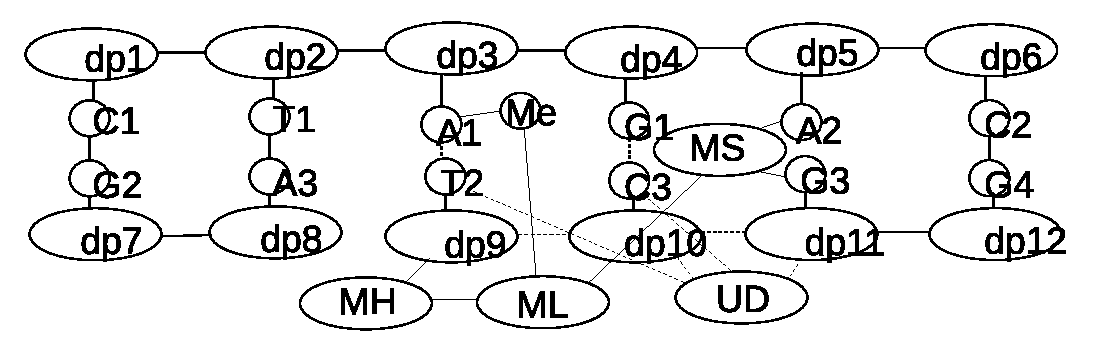
\includegraphics[width=1.0\textwidth]{mmr/state3}
  \caption[A six base pair DNA fragment.]{%A six base pair DNA fragment, with a DNA mismatch and methylation of one strand.
  $\UvrD$ has now bonded to $T_2$ and $\DP_{10}$ (blue lines), thus breaking the bonds of  the $DP_9$-$T_2$ group to the rest of the DNA (red dotted lines). %In a next step, $\UvrD$ can now ``walk'' along the DNA strand, and remove the next pair of $\DP$ and base molecules.
}
  \label{fig:state3}
\end{figure}

$\UvrD$ can now ``walk'' along the lower chain of the strand towards the right end.
%As opposed to BER, the bonds between the base pairs are now broken during the walk.
Concurrently, the bonds between the deoxyribose/phosphate groups are also broken as $\UvrD$ progresses. We write these reactions as two separate sequences of transitions for clarity, with the first transition in full, and note that this is the place
where could have used the shortcut  \rulename{concert3} SOS rule.
\begin{flalign*}
& (b_1[6];i_1).(a_1,m_1[40];r_1).A_1' \paral  (b_6[9];i_6).(g_1[25];r_6).G_1' \paral &&\\
&(b_2[7];i_2).(a_2[28],m_2;r_2).A_2' \paral (b_5[19];i_5).(t_2[35]; r_5).T_2' \paral (b_{12}[20];i_{12}).(c_3[25];r_{12}).C_3'  \paral&&\\
&(b_8[21];i_8).(g_3[29];r_8).G_3' \paral ((p3_8[12],p5_8[33];s_8) \paral (b_8[18],d_8)).\DP_8' \paral &&\\
&((p3_9,p5_9;s_9) \paral (b_9[19],d_9)).\DP_9' \paral ((\Red{\bm{p3_{10}[34]}},\Red{\bm{p5_{10}[15]}};s_{10}) 
 \paral (b_{10}[20],d_{10})).\DP_{10}' \paral  &&\\
&((\Red{\bm{p3_{11}[15]}},p5_{11}[16];\Blue{\bm{s_{11}}}) \paral (b_{11}[21],d_{11})).\DP_{11}' \paral ((p3_{12}[16],p5_{12};s_{12}) \paral (b_{12}[22],d_{12})).\DP_{12}' \paral  &&\\
&(m[40]).(n[31]).\Me'\paral (k[28],k[29]).(l[30]).\MutS' \paral (l[30]).(n[31]).(o[32]).\MutL' \paral &&\\
&(o[32]).(w[33]).\MutH' \paral ((u[35];r) \paral (\Red{\bm{v[34]}};\Blue{\bm{s}})).\UvrD'&&\\
%
& \xxrightarrow{\{ss[36],\underline{vp3}[34]} \; \xxrightarrow{\underline{p}[15]}\\
%&\xrightarrow{\{ss[36],\underline{vp3}[34],\underline{p}[15]\}}
%\overset{ \rulename{prom}}\Rightarrow \; \overset{ \rulename{prom}}\Rightarrow\\
%
& (b_1[6];i_1).(a_1,m_1[40];r).A_1' \paral (b_6[9];i_6).(\Red{\bm{g_1[25]}};r_3).G_1' \paral &&\\
&(b_2[7];i_2).(a_2[28],m_2;r).A_2' \paral (b_5[19];i_5).(\Red{\bm{t_2[35]}};r_2).T_2' \paral (b_{11}[20];i_{11}).(\Red{\bm{c_3[25]}};\Blue{\bm{r_8}}).C_3'  \paral&&\\
&(b_8[21];i_8).(g_2[29];r_4).G_3' \paral ((p3_8[12],p5_8[33];s_8) \paral (b_8[18],d_8)).\DP_8' \paral &&\\
&((p3_9,p5_9;s_9) \paral (b_9[19],d_9)).\DP_9' \paral ((\bm{p3_{10},p5_{10}};s_{10}) \paral (b_{10}[20],d_{10})).\DP_{10}' \paral &&\\
&((\bm{p3_{11}[36]},p5_{11}[16];\bm{s_{11}}) \paral (b_{11}[21],d_{11})).\DP_{11}' \paral ((p3_{12}[16],p5_{12};s_{12}) \paral (b_{12}[22],d_{12})).\DP_{12}' \paral  &&\\
&(m[40]).(n[31]).\Me'\paral (k[28],k[29]).(l[30]).\MutS' \paral (l[30]).(n[31]).(o[32]).\MutL' \paral &&\\
&(o[32]).(w[33]).\MutH' \paral ((\Red{\bm{u[35]}};\Blue{\bm{r}}) \paral (\bm{v[36]};\bm{s})).\UvrD'&&
\end{flalign*}
Notice that promotion has moved a bond from $s_{11}$ to $p3_{11}$ and from $s$ to $v$. Instead of using these
transitions we could have applied \rulename{concert3}, we could have used this sequence of transitions from the source to the target process:
$\xrightarrow{\{ss[36],\underline{vp3}[34],\underline{p}[15]\}}
\overset{ \rulename{prom}}\Rightarrow \; \overset{ \rulename{prom}}\Rightarrow$.

Next,  $\UvrD$ combines with $C_3$ thus breaking bonds with keys 35 and 25. 
\begin{flalign*}
& \xxrightarrow{\{rr[37],\underline{tu}[35]\}}\; \xxrightarrow{\underline{cg}[25]}
%&\xrightarrow{\{rr[37],\underline{tu}[35],\underline{cg}[25]\}}
%\overset{ \rulename{prom}}\Rightarrow \; \overset{ \rulename{prom}}\Rightarrow
 (b_1[6];i_1).(a_1,m_1[40];r).A_1' \paral (b_6[9];i_6).(\bm{g_1};r_3).G_1' \paral  &&\\
&(b_2[7];i_2).(a_2[28],m_2;r).A_2' \paral (b_5[19];i_5).(\bm{t_2};r_2).T_2' \paral (b_{11}[20];i_{11}).(\bm{c_3[37]};\bm{r_8}).C_3'  \paral&&\\
&(b_8[21];i_8).(g_2[29];r_4).G_3' \paral  ((p3_8[12],p5_8[33];s_8) \paral (b_8[18],d_8)).\DP_8' \paral &&\\
&((p3_9,p5_9;s_9) \paral (b_9[19],d_9)).\DP_9' \paral ((p3_{10},p5_{10};s_{10}) \paral (b_{10}[20],d_{10})).\DP_{10}' \paral &&\\
&((p3_{11}[36],p5_{11}[16];s_{11}) \paral (b_{11}[21],d_{11})).\DP_{11}' \paral ((p3_{12}[16],p5_{12};s_{12}) \paral (b_{12}[22],d_{12})).\DP_{12}' \paral  &&\\
&(m[40]).(n[31]).\Me'\paral (k[28],k[29]).(l[30]).\MutS' \paral (l[30]).(n[31]).(o[32]).\MutL' \paral &&\\
&(o[32]).(w[33]).\MutH' \paral ((\bm{u[37]};\bm{r}) \paral (v[36];s)).\UvrD'&&
\end{flalign*}
Promotion moves bonds from
$r_8$ to $c_3$ and from $r$ to $u$ below.
Correspondingly as above, we could use shortcut rule \rulename{concert3} and write these reactions
using this sequence: $\xrightarrow{\{rr[37],\underline{tu}[35],\underline{cg}[25]\}}
\overset{ \rulename{prom}}\Rightarrow \; \overset{ \rulename{prom}}\Rightarrow$.


The resulting system is shown in Figure~\ref{fig:state4}. Here, the first  base $T_2$ and deoxyribose/phosphate group
$\DP_9$ have been removed (shown in grey) and $\UvrD$ has moved to the next  base $C_3$
and deoxyribose/phosphate group $\DP_{10}$, again to remove them. The two concerted actions transitions that represent these reactions are with the keys (36,34,15) and (37,35,25) respectively.
%Notice that here we have used the new rule \rulename{concert 3}.

\begin{figure}[h!]
\psfrag{25}[cc][][0.8][0]{$25$}
\psfrag{15}[cc][][0.8][0]{$15$}
\psfrag{35}[cc][][0.8][0]{$35$}
\psfrag{34}[cc][][0.8][0]{$34$}
\psfrag{36}[cc][][0.8][0]{$36$}
\psfrag{37}[cc][][0.8][0]{$37$}
\psfrag{dp1}{${DP_1}$}
\psfrag{dp2}{${DP_2}$}
\psfrag{dp3}{${DP_3}$}
\psfrag{dp4}{${DP_4}$}
\psfrag{dp5}{${DP_5}$}
\psfrag{dp6}{${DP_6}$}
\psfrag{dp7}{${DP_7}$}
\psfrag{dp8}{${DP_8}$}
\psfrag{dp9}{\color{gray}${DP_9}$}
\psfrag{dp10}{${DP_{10}}$}
\psfrag{dp11}{${DP_{11}}$}
\psfrag{dp12}{${DP_{12}}$}
\psfrag{A1}[cc][][0.8][0]{${A_1}$}
\psfrag{A2}[cc][][0.8][0]{${A_2}$}
\psfrag{A3}[cc][][0.8][0]{${A_3}$}
\psfrag{T1}[cc][][0.8][0]{${T_1}$}
\psfrag{T2}[cc][][0.8][0]{\color{gray}${T_2}$}
\psfrag{C1}[cc][][0.8][0]{${C_1}$}
\psfrag{C2}[cc][][0.8][0]{${C_2}$}
\psfrag{C3}[cc][][0.8][0]{${C_3}$}
\psfrag{G1}[cc][][0.8][0]{${G_1}$}
\psfrag{G2}[cc][][0.8][0]{${G_2}$}
\psfrag{G3}[cc][][0.8][0]{${G_3}$}
\psfrag{G4}[cc][][0.8][0]{${G_4}$}
\psfrag{Me}{${\mathit{Me}}$}
\psfrag{MS}{${\mathit{MutS}}$}
\psfrag{ML}{${\mathit{MutL}}$}
\psfrag{MH}{${\mathit{MutH}}$}
\psfrag{UD}{${\mathit{UvrD}}$}
  \centering
    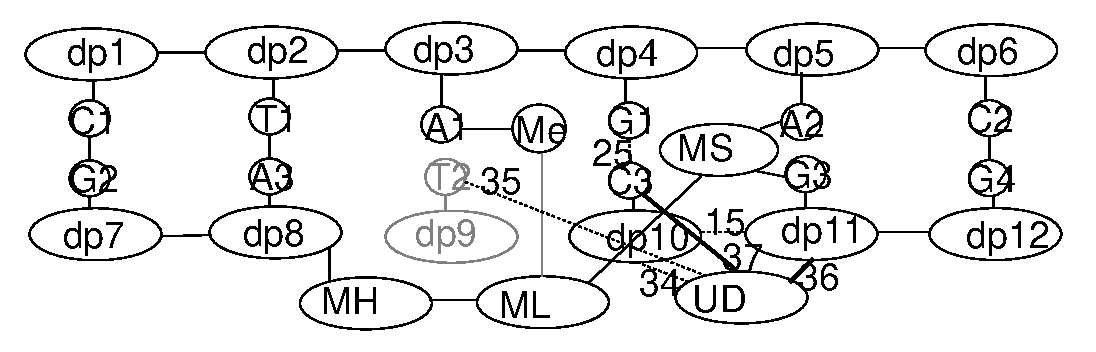
\includegraphics[width=1.0\textwidth]{mmr/state4}
  \caption[A six base pair DNA fragment.]{%A six base pair DNA fragment, with a DNA mismatch and methylation of one strand.
  $\UvrD$ has now bonded to $C_3$ and $\DP_{11}$, thus breaking the bonds of the $DP_{10}$-$C_3$ group with the rest of the DNA (via two concerted actions). The $T_2$-$\DP_{9}$ group is no longer attached to the DNA (shown in grey). % This process can continue for more pairs.
}
  \label{fig:state4}
\end{figure}

This process continues until the offending base $G_3$ has been removed. We do not show concerted actions transitions that model this since they correspond very closely to the last two transitions. Figure~\ref{fig:state6} shows the result of these two transitions which remove of the offending base.
%We do not model how the number of base pairs to remove is determined.
%In reality, that number is not fixed, but is determined by the interal workings of the protein, where the number is statistically distributed.
Once this is done and the $\MutH$, $\MutL$, and $\MutS$ proteins have detached we get the situation shown in Figure~\ref{fig:state7}.


\begin{figure}[t!]
\psfrag{29}[cc][][0.8][0]{$29$}
\psfrag{16}[cc][][0.8][0]{$16$}
\psfrag{38}[cc][][0.8][0]{$38$}
\psfrag{39}[cc][][0.8][0]{$39$}
\psfrag{36}[cc][][0.8][0]{$36$}
\psfrag{37}[cc][][0.8][0]{$37$}
\psfrag{dp1}{${DP_1}$}
\psfrag{dp2}{${DP_2}$}
\psfrag{dp3}{${DP_3}$}
\psfrag{dp4}{${DP_4}$}
\psfrag{dp5}{${DP_5}$}
\psfrag{dp6}{${DP_6}$}
\psfrag{dp7}{${DP_7}$}
\psfrag{dp8}{${DP_8}$}
\psfrag{dp9}{${DP_9}$}
\psfrag{dp10}{\color{gray}${DP_{10}}$}
\psfrag{dp11}{${DP_{11}}$}
\psfrag{dp12}{${DP_{12}}$}
\psfrag{A1}[cc][][0.8][0]{${A_1}$}
\psfrag{A2}[cc][][0.8][0]{${A_2}$}
\psfrag{A3}[cc][][0.8][0]{${A_3}$}
\psfrag{T1}[cc][][0.8][0]{${T_1}$}
\psfrag{T2}[cc][][0.8][0]{${T_2}$}
\psfrag{C1}[cc][][0.8][0]{${C_1}$}
\psfrag{C2}[cc][][0.8][0]{${C_2}$}
\psfrag{C3}[cc][][0.8][0]{\color{gray}${C_3}$}
\psfrag{G1}[cc][][0.8][0]{${G_1}$}
\psfrag{G2}[cc][][0.8][0]{${G_2}$}
\psfrag{G3}[cc][][0.8][0]{${G_3}$}
\psfrag{G4}[cc][][0.8][0]{${G_4}$}
\psfrag{Me}{${\mathit{Me}}$}
\psfrag{MS}{${\mathit{MutS}}$}
\psfrag{ML}{${\mathit{MutL}}$}
\psfrag{MH}{${\mathit{MutH}}$}
\psfrag{UD}{${\mathit{UvrD}}$}
  \centering
    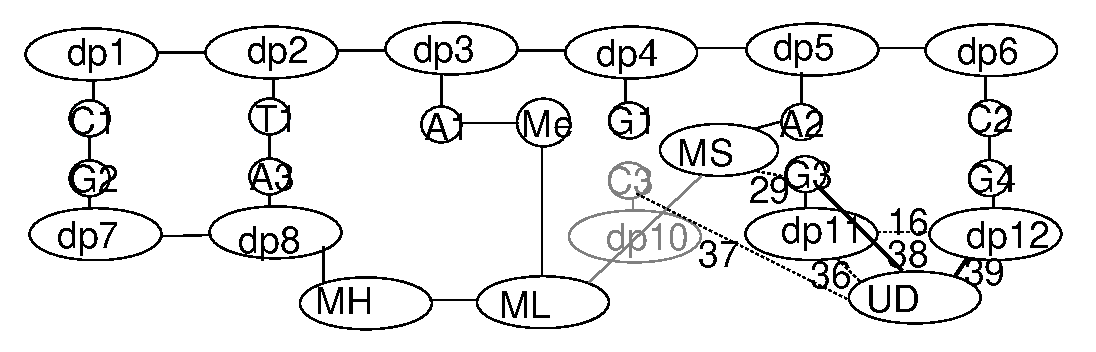
\includegraphics[width=1.0\textwidth]{mmr/state6}
  \caption[A six base pair DNA fragment.]{%A six base pair DNA fragment, with a DNA mismatch and methylation of one strand.
$\UvrD$ has now bonded to $G_3$ (the offending base) and $\DP_{12}$, thus breaking the bonds of the 
$G_3$-$DP_{11}$ group to the rest of the DNA (via two concerted actions). The $C_3$-$\DP_{10}$ group is now removed (shown in grey). Next, the group $G_3$-$DP_{11}$ will be removed.}
  \label{fig:state6}
\end{figure}

\begin{figure}[]
\psfrag{dp1}{${DP_1}$}
\psfrag{dp2}{${DP_2}$}
\psfrag{dp3}{${DP_3}$}
\psfrag{dp4}{${DP_4}$}
\psfrag{dp5}{${DP_5}$}
\psfrag{dp6}{${DP_6}$}
\psfrag{dp7}{${DP_7}$}
\psfrag{dp8}{${DP_8}$}
\psfrag{dp9}{${DP_9}$}
\psfrag{dp10}{${DP_{10}}$}
\psfrag{dp11}{${DP_{11}}$}
\psfrag{dp12}{${DP_{12}}$}
\psfrag{A1}[cc][][0.8][0]{${A_1}$}
\psfrag{A2}[cc][][0.8][0]{${A_2}$}
\psfrag{A3}[cc][][0.8][0]{${A_3}$}
\psfrag{T1}[cc][][0.8][0]{${T_1}$}
\psfrag{T2}[cc][][0.8][0]{${T_2}$}
\psfrag{C1}[cc][][0.8][0]{${C_1}$}
\psfrag{C2}[cc][][0.8][0]{${C_2}$}
\psfrag{C3}[cc][][0.8][0]{${C_3}$}
\psfrag{G1}[cc][][0.8][0]{${G_1}$}
\psfrag{G2}[cc][][0.8][0]{${G_2}$}
\psfrag{G3}[cc][][0.8][0]{${G_3}$}
\psfrag{G4}[cc][][0.8][0]{${G_4}$}
\psfrag{Me}{${\mathit{Me}}$}
\psfrag{MS}{${\mathit{MutS}}$}
\psfrag{ML}{${\mathit{MutL}}$}
\psfrag{MH}{${\mathit{MutH}}$}
\psfrag{UD}{${\mathit{UvrD}}$}
  \centering
    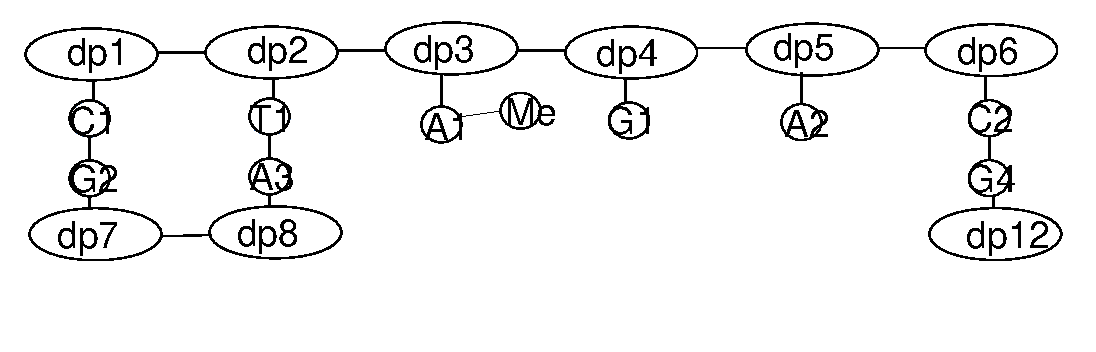
\includegraphics[width=1.0\textwidth]{mmr/state7}\vspace{-1cm}
  \caption[A six base pair DNA fragment.]{A DNA fragment with a gap of three bases in one strand produced by MMR.}
  \label{fig:state7}
\end{figure}
The resulting system is now ready for other proteins to replace the bases and deoxyribose/phosphate groups. Notice that the remaining strand contains the necessary information for this, in particular that only a $T$ base can bond with $A_1$ and $A_2$ and that a $C$ must bond with $G_1$. Note that the methyl group stays attached to $A_1$, since it is still an old DNA strand. Also the appropriate groups in the new, lower half will be methylated, so that both strands are marked as old material after the next DNA duplication process.

\subsection{Evaluation}

We have shown that CCB can be used to model the MMR gene repair mechanism. This is significant since the calculus was designed for simpler lower level systems and reactions. We have been able to reuse the main features of CCB, in particular, the concerted actions. Out-of-causal order reversibility plays a significant role in our example, in particular for the modelling of movement of the proteins along the DNA chain.

There is one aspect of our reactions which we model adequately but which we intend to improve in the future. This is the breaking of two bonds as a result of one bond on weak actions being formed as, for example, in these transitions   $\xrightarrow{\{rr[37],\underline{tu}[35],\underline{cg}[25]\}}
\overset{ \rulename{prom}}\Rightarrow \; \overset{ \rulename{prom}}\Rightarrow$ derived with the  shortcut  \rulename{concert3} rule. Currently, we represent this
by two consecutive transitions $\xxrightarrow{\{rr[37],\underline{tu}[35]\}}\; \xxrightarrow{\underline{cg}[25]}$, but note 
that these transitions can be interleaved by other transitions, which weakens the modelling of the two bonds being broken immediately after the weak bond is created. In short, our \rulename{concert} rules, which were developed for covalent reactions, are not general enough.

% In contrast to the real situation, this rule does not link the breaking of the second bond directly to the formation of the new bond. Here, the  \rulename{concert} rule, which was derived from how covalent reactions work, is not general enough.

Our calculus permits the modelling of certain reactions which normally do not happen in reality, and this property is inherited from the original CCB. This is mainly due to non-consideration of aspects of spatial configuration of proteins and bases. We give several examples of reactions where do not model the spacial aspect adequately: 
\begin{itemize}
\item We have not modelled the formation of the loop in the DNA, which is crucial for cleaving the correct strand. In reality, 
$\MutL$ forms a loop in the strand, which hides the methylated strand, making sure in this way that $\MutH$ cleaves the un-methylated (meaning new) strand.
\item In our model, $\MutL$ can bond to any methyl group and a base pair any distance apart. In reality, $\MutL$ has 
a fixed size and it can only react with parts of the DNA it can physically reach. Similarly, $\UvrD$ can bond to any deoxyribose/phosphate group, not just the neighbouring one. 
\end{itemize}

We have checked that all reactions given in this section are possible in our model by using the simulation software tool~\cite{10.1007/978-3-319-99498-7_8}, which has been extended to cover the extended prefix operator.

%
\section{Conclusion}

We have shown previously that the Calculus of Covalent Bonding can be used successfully to represent and simulate higher-level biochemical processes and reactions. In this paper, we have used the calculus to model an important gene repair pathway, namely the DNA Mismatch Repair (MMR) mechanism. We have extended the calculus with a prefix operator that can represent multiple bonding sites. We have also included a shorthand notation for concerted actions transitions, involving three actions, which, strictly speaking, does not represent an extension of the calculus.

The MMR mechanism is a complex pathway. We have modelled it with twelve deoxyribose/phosphate groups, twelve bases and four helper proteins, all composed in parallel. We then have shown a sequence of transitions (representing bonding reactions and cascades of concerted reactions with either two or three reactions each) that represent the MMR mechanism. As shown, the shortcut rule \rulename{concert3} is only an approximation of reality. Also, we have not been able to consider some spatial aspects of such reactions in the current setting, which is left to future research. Overall, we still were able to demonstrate the general use of CCB outside its immediate domain.

\bibliography{mybibfile}

\end{document}